%!TEX program = lualatex
\documentclass[a4paper]{article}
\usepackage[margin=2cm]{geometry}
\usepackage{multicol}
\usepackage[hyphens]{url}
\usepackage[swedish]{babel}
\usepackage[hidelinks]{hyperref}
\usepackage{dirtytalk}
\usepackage{qrcode}
\usepackage{tabularx}
\usepackage{calc}
\usepackage{fancyhdr}
\usepackage{fontspec}
\usepackage{etoolbox}
\usepackage{forloop}

%\let\oldqrcode\qrcode
%\renewcommand{\qrcode}[1]{\parbox[b][1cm]{1cm}{\oldqrcode{#1}}}

\pagestyle{fancy}
\fancyhf{}
\renewcommand{\headrulewidth}{0.0pt}
\cfoot{\thepage\\
{\tiny Skriv ut en kopia av detta dokument: \href{http://goo.gl/vbce1U}{goo.gl/vbce1U} - \today}}
\newfontfamily\Emoji{OpenSansEmoji}

\makeatletter

\directlua{

function url_encode(str)
  if (str) then
    str = string.gsub (str, "\string\n", "\string\r\string\n")
    str = string.gsub (str, "([^\@percentchar w \@percentchar -\@percentchar _\@percentchar .\@percentchar \string~])",
        function (c) return string.format ("\@percentchar \@percentchar \@percentchar 02X", string.byte(c)) end)
    str = string.gsub (str, " ", "+")
  end
  return str
end

function twitterify(str)
	print("===============================================\string\n")
	str = string.gsub(str, "@(\@percentchar w+)", "\string\\href{http://twitter.com/\@percentchar1}{@\@percentchar1}")
	str = string.gsub(str, "\string\\\string#([\@percentchar wåäöÅÄÖ_]+)", function(a) return "\string\\href{http://twitter.com/hashtag/" .. url_encode(a) .. "}{\string\\\string#" .. string.gsub(a, "\string_", "\string\\_") .. "}" end)
	print(str)
	print("===============================================\string\n")
	return str
end
}

\newcounter{entrycnt}
\newcommand\addentry[4]{
  \stepcounter{entrycnt}
  \csdef{title\theentrycnt}{#1}
  \csdef{preamble\theentrycnt}{\directlua{tex.print(twitterify([==[\detokenize{#2}]==]))}}
  \csdef{url\theentrycnt}{#3}
  \csdef{extras\theentrycnt}{#4}
}
\newcommand{\entry}{
\catcode`\%=12
\@entry}
\newcommand{\@entry}[4][]{
\addentry{#2}{#3}{#4}{#1}
\catcode`\%=14
}

\newcommand\makeentry[1]{
	\bigskip
	\begin{tabular*}{\textwidth}{l m{\textwidth-4cm}}
	\qrcode{\csuse{url#1}} & \textbf{\csuse{title#1}}

	\medskip

	\url{\csuse{url#1}}

	\end{tabular*}

	\medskip


	\begin{multicols}{2}
	\csuse{preamble#1}
	\end{multicols}

	\csuse{extras#1}

	\medskip
	\hrule
}
\makeatother


\begin{document}

{
\LARGE Skriv ut detta dokument:

\bigskip

\begin{tabular*}{\textwidth}{l m{\textwidth-4cm}}
\qrcode{http://arneweisse.github.io/samling/samling.html} & \url{http://arneweisse.github.io/samling/samling.html} \\
\\
\qrcode{https://github.com/arneweisse/samling/raw/master/samling.pdf} & \url{https://github.com/arneweisse/samling/raw/master/samling.pdf} \\
\\
\qrcode{http://github.com/arneweisse/samling} & \url{http://github.com/arneweisse/samling} \\
\end{tabular*}
}



\begin{multicols}{2}

Detta dokument samlar läkares, patienters, funktionsnedsattas och kritikers röster om sjukförsäkringen och LSS. De allra flesta texter är daterade september till december 2017.

Kodrutan bredvid alla länkar är en så kallad QR-kod, från engelskans \say{Quick Response}. Den fungerar ungefär som streckkoderna på varor i mataffären. Genom ett gratisprogram i mobilen kan man skanna koden med hjälp av mobilens kamera och på så sätt slippa skriva in länkadressen själv. Sök i din mobils \say{app-store} efter \say{QR} så får du en lista på olika gratisprogram. Efter att man har skannat in koden kan man själv välja om man vill öppna länken eller ej.

Alla QR-koder i detta dokument motsvarar alltid exakt den länkadress som står bredvid den.

I den digitala versionen av detta dokument, som återfinns på ovanstående länkar, är alla länkar klickbara.

Skriv ut en kopia, twittra, dela och diskutera med vänner och kollegor! Sjukdom, hjärnskador, stroke m.m. kan drabba alla människor, även dig själv och dina närmsta.

\end{multicols}

\medskip
\hrule

\entry{20 juni 2010 - Kritiker: Staten bryter mot lagen}{
Socialförsäkringar som till exempel sjukpenningen beskrivs ofta som stora kostnader för staten. Men tvärtom mot vad många tror så tjänar statskassan miljarder på försäkringarna – varje år.

Förklaringen är att staten tar ut mycket mer i avgift för socialförsäkringen än vad som betalas ut till kunderna ? det vill säga folket. Det är fel, menar kritikerna.}
{https://www.svt.se/nyheter/inrikes/kritiker-staten-bryter-mot-lagen?cmpid=del:tw:20171021:kritiker-staten-bryter-mot-lagen:nyh:lp}


\entry{14 dec 2010 - Försäkringskasseutlöst stupor vid Aspergers syndrom}{De strängare reglerna för sjukersättning drabbar psykiatrins patienter hårt. Artikelförfattarna illustrerar detta med ett fall från den kliniska verkligheten. De fäster samtidigt läsarnas uppmärksamhet på att individer med neuropsykiatriska handikapp kan gå in i allvarliga stuporösa tillstånd vid stress.}{http://www.lakartidningen.se/Functions/OldArticleView.aspx?articleId=15656}

\entry{4 augusti 2016 - Kompetens och kapacitet - konsekvenser av att inte skilja begreppen åt}{Person 1 har hög kapacitet men låg kompetens i förhållande till den förväntade nivån. Hen är alltså underkvalificerad för arbetet trots sin höga kapacitet. Person 2 har däremot låg kapacitet men hög kompetens i förhållande till den förväntade nivån. Hen är istället överkvalificerad för arbetet trots sin låga kapacitet.

När vi ser det så här blir det tydligt att det inte går att hjälpa dessa två personer på samma sätt. För att kunna utföra arbetet behöver person 1 öka sin kompetens, eller så får arbetsgivaren sänka sina krav på kompetens. För att person 2 ska kunna utföra samma arbete behöver hen öka sin kapacitet eller så får arbetsgivaren sänka kraven på kapacitet.

Att sänka kraven på kompetens sänker inte automatiskt kraven på kapaciteten och att sänka kraven på kapacitet sänker inte automatiskt kraven på kompetensen. De är variabler som är helt oberoende av varandra samtidigt som kapaciteten väldigt tydligt påverkar hur mycket en person kan utnyttja sin kompetens.

Den som tror att nivån på kapacitet styr nivån på komptenens och vice versa blir väldigt förvirrad av att träffa en person med hög kompetens som har mycket låg kapacitet.}{http://livetsbilder.blogspot.se/2016/08/kompetens-och-kapacitet-konsekvenser-av.html}


\entry{13 februari 2017 - Utbrända Malin blev utan sjukpenning}{Allt fler nekas sjukpenning eller får den indragen. Det visar siffror från Försäkringskassan.}{https://www.svt.se/nyheter/lokalt/vasterbotten/utbranda-malin-blev-utan-sjukpenning}

\entry{14 februari 2017 - Forskare riktar hård kritik mot Försäkringskassan}{Jag skulle vilja se att man lägger mer fokus på att ta reda på varför man hamnar i sjukförsäkring innan man slänger ut folk ur försäkringen}{https://www.svt.se/nyheter/lokalt/vasterbotten/fler-nekas-sjukpenning-forskare-kritisk}

\entry{14 feb 2017 - Den dolda sjukfrånvaron växer}{Nyligen pratade jag med A, en undersköterska som fått sin sjukpenning på deltid indragen av Försäkringskassan (FK). Hon valde då, i samråd med arbetsgivaren, att omvandla sin heltidsanställning till en deltidstjänst.

Hon orkade inte längre bråka med FK, trots att hennes läkare och arbetskamrater tycker hon borde stå på sig och begära omprövning. \say{Min 80-åriga mamma ligger för döden och jag är hennes enda stöd. Jag orkar inte samtidigt slåss mot FK}, sa hon.}{http://www.nsd.se/nyheter/den-dolda-sjukfranvaron-vaxer-nm4452835.aspx}


\entry{15 feb 2017 - Min (o)tur nu?}{Så­ efter sex års sjukskrivning, 27 läkarintyg utan anmärkning och noll tvekan från någon om att jag har behov av att vara sjukskriven ­ så duger helt plötsligt inte det underlag som finns. Och utifrån ett ofullständigt läkarintyg drar de alltså slutsatsen att jag inte längre saknar arbetsförmåga.}{http://livetsbilder.blogspot.se/2017/02/min-otur-nu.html}

\entry{16 feb 2017 - Sjukskrivning – en process för att förnedra och skrämma människor ur sjukförsäkringen?}{Efter en dryg månad kom det ett brev från Försäkringskassan som verkade vara en kopia på ett brev handläggaren hade skickat till den sjukskrivande läkaren. Brevet innehöll information om att intyget behövde kompletteras. Jag bröt ihop, grät och sov sämre en vanligt de kommande nätterna. Det mesta som handläggaren begärde komplettering om fanns i intyget, ändå hade FMR menat att det behövde förtydligas.}{https://funkisfeministen.wordpress.com/2017/02/16/sjukskrivning-en-process-for-att-fornedra-och-skramma-manniskor-ur-sjukforsakringen/}

\entry{16 feb 2017 - Läkarförbundet: \say{Vårdkedjan haltar}}{\say{En patient mår inte bättre av att bråka med försäkringskassan}, säger Robert Svartholm, huvudskyddsombud i Norrbottens läkarförbund, är kritisk.

– Jag blir förvånad att försäkringskassan får ökande resurser och granskar våra intyg mer utförligt utan att prata med oss. Det innebär i klartext att vårdkedjan haltar. Om de får utökade resurser och vi får sämre resurser så blir det naturligtvis ett ökat gap mellan oss, och då kommer patienterna i kläm, säger Robert Svartholm.

Sjukintygen har fått stor uppmärksamhet den senaste tiden efter att en insändare publicerades i NSD och Kuriren. En läkare upplever en problematisk situation där försäkringskassan bedömer att en patient kan jobba, medan hon har skrivit motsatsen i sjukintyget. Robert Svartholm känner igen sig i situationen som läkaren beskriver i sin insändare.

– Många av oss läkare delar hennes uppfattning och upplevelser. Vi är mer eller mindre upprörda.

Han berättar att läkarförbundet på central nivå har haft kontakt med försäkringskassan för att prata om hanteringen av sjukintyg, men att samarbetet inte fungerat.

– Jag vet att läkarförbundet har varit kritiskt till försäkringskassans agerande, säger han.}{http://www.nsd.se/nyheter/lakarforbundet-vardkedjan-haltar-nm4455997.aspx}

\entry{16 feb 2017 - Nu har jag fått nog av Försäkringskassan}{En av mina patienter har fått avslag upprepade gånger eftersom FK inte tycker att hon har en nedsatt arbetsförmåga ens med 25 procent, medan min bedömning är att hon i dagsläget inte klarar av att ta något vanligt jobb på arbetsmarknaden alls. Efter det sista nekandet blev jag så arg att jag skrev till FK och begärde ett möte. Någon vecka senare fick jag svaret att FK bedömde att de hade all information som behövdes och att det därför inte skulle bli något möte.

Om nu handläggarna på FK tycker att vi som doktorer, med minst sju års yrkesutbildning (tolv år om du är specialist), inte är kompetenta nog att göra en bedömning om en person har arbetsförmåga eller inte, undrar jag varför vi över huvudtaget ska delta i sjukskrivningsprocessen?}{http://www.kuriren.nu/opinion/nu-har-jag-fatt-nog-av-forsakringskassan-nm4454792.aspx}

\entry{27 feb 2017 - \say{De har en tro på att all sjukdom syns i rummet}}{Kafkaartade situationer där hon gång på gång avkrävs statusfynd som inte finns. Sjukhusläkaren bad företagsläkaren och reumatologen Ylva Rangnitt ge tre omöjliga exempel från sin vardagliga kommunikation med Försäkringskassan.}{http://www.sjukhuslakaren.se/de-har-en-tro-pa-att-all-sjukdom-syns-i-rummet/}

\entry{24 mar 2017 - Hur skall man bli frisk utan pengar?}{Nu har försäkringskassan börjat tillämpa hårdare bedömningar av de som lider av diagnoserna utmattningssyndrom och depression.
Det innebär att de medicinska intyg som för mindre än ett halvår sedan räckte för att garantera inkomst i form av sjukpenning, idag avslås med formuleringen; ”Det medicinska underlaget styrker inte arbetsförmågenedsättning med minst 25 procent”. Samma intyg, samma medicinska lidande men en helt annan tolkning från försäkringskassans sida.}{http://www.pt.se/opinion/debatt/hur-skall-man-bli-frisk-utan-pengar-10483418.aspx}

\entry{6 Apr 2017}{Försäkringskassan skärpte reglerna – Nu tvingas funktionsnedsatta barn ligga månader på sjukhus}{https://nyheteridag.se/forsakringskassan-skarpte-reglerna-nu-tvingas-funktionsnedsatta-barn-ligga-i-manader-pa-sjukhus/}

\entry{16 maj 2017 - Strandhäll smyger in en ny stupstock}{Socialförsäkringsminister Annika Strandhäll har satt upp målet att få ner sjukpenningtalet från dagens 10,8 dagar till nio dagar till 2020.
För drygt ett år sedan togs den bortre tidsgränsen i sjukförsäkringen bort. Det beskrevs som en seger och var en av Socialdemokraternas största stridsfrågor under förra valrörelsen. Men resultatet av de hårdare bedömningarna av läkarintygen har i verkligheten lett till att vi fått en ny stupstock.
Ännu en gång ser vi hur långvarigt sjuka blir ekonomiskt beroende av nära anhörig eller tvingas söka försörjningsstöd.}{https://www.aftonbladet.se/ledare/a/eQBqQ/strandhall-smyger-in-en-ny-stupstock}

\entry{24 maj 2017}{\#jagsaknas i statistiken. Sjuk men ingen sjukpenning sedan dec -16. \#mecfs}{https://twitter.com/radioprofil/status/867466418459115520}

\entry{28 maj 2017}{Ableism innebär att människor med funktionsnedsättningar värderas lägre än människor utan funktionsnedsättningar.}{https://twitter.com/Jonna_A/status/868822679780044800}


\entry{30 maj 2017 - \say{LSS faller sönder – dags att dra i nödbromsen}}{Familjer med små barn står skyddslösa. Unga vuxna som är på väg ut i livet kommer inte vidare. Den välfärd som vi tagit för given vacklar därför att en av de bärande pelarna fallit sönder. Funktionsrätt Sverige kräver nu att riksdagen sätter stopp för den pågående utvecklingen när det gäller LSS och insatsen personlig assistans.}{https://www.dagenssamhalle.se/debatt/lss-faller-sonder-dags-att-dra-i-nodbromsen-17379}

\entry{3 jun 2017 - Sverige blir friskare! Eller?}{Vi kan alltså konstatera att när regeringen satte ett mål på 9 sjukdagar per år, gav det genast effekten att Försäkringskassan avslog fler ansökningar.

Utvecklingen går alltså åt det håll politikerna önskar. Men på ett sätt som ingen (förhoppningsvis) önskar: genom att färre av de som läkare bedömer behöver sjukskrivning, får det.

Socialförsäkringsminister Annika Strandhäll är dock inte nöjd. Såklart hon inte är! Socialdemokraterna har ju alltid stått upp för ett starkt socialt skyddsnät!

Nej, alltså \ldots hon är inte missnöjd med avslagen. Hon är missnöjd med att det är fortfarande är så många som får sjukpenning – speciellt kvinnor}{http://tankesmedjanbalans.se/sjuktal/}

\entry[{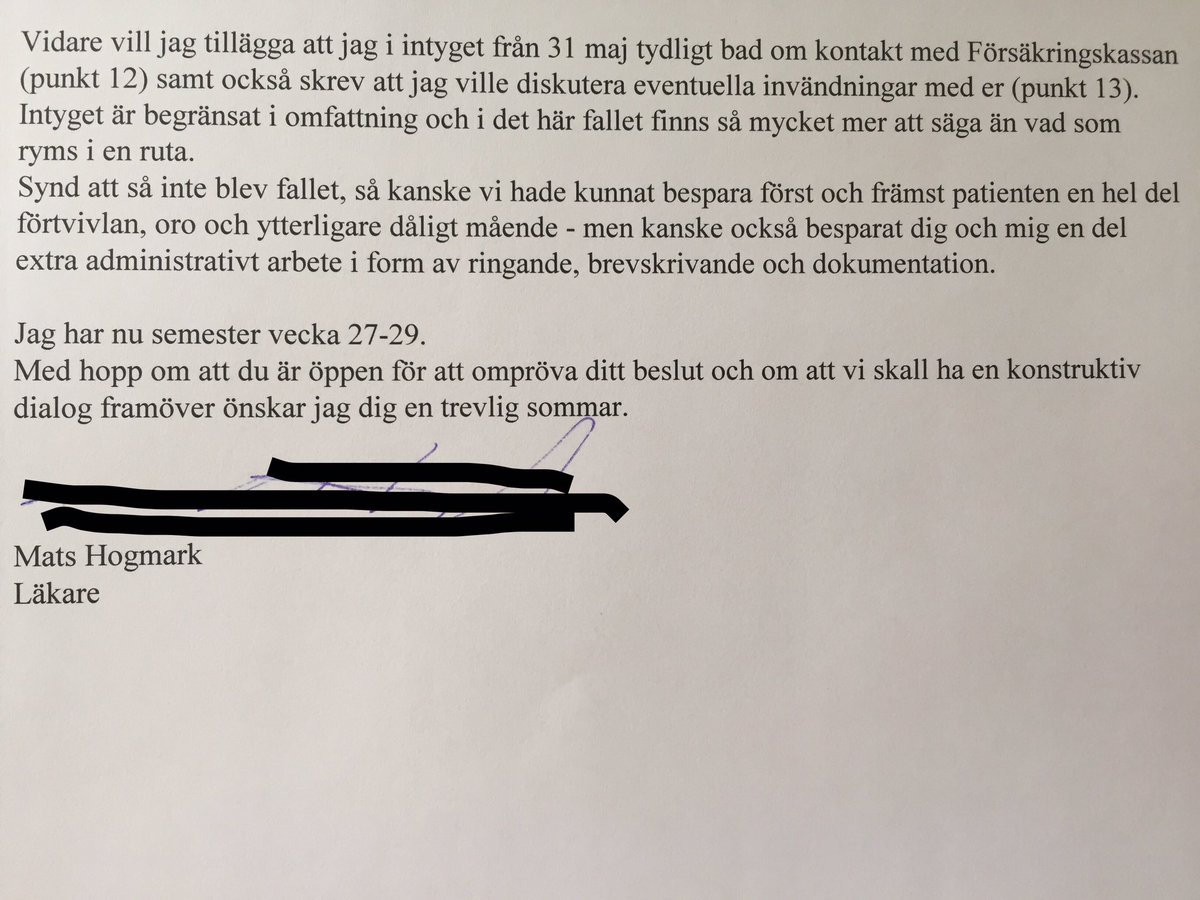
\includegraphics[width=\textwidth,height=\textheight,keepaspectratio]{879267487245885440.jpg}}]{26 jun 2017}{Del av min interaktion med  \#försäkringskassan idag. Jag blir galen!
Och som vanligt hamnar patienten mest i kläm\ldots}{https://twitter.com/matshogmark/status/879267487245885440}

\entry{3 jul 2017 - Systemet slår hårt mot personer med psykisk sjukdom}{Den psykiska ohälsan ökar i samhället. Samtidigt drar Försäkringskassan in sjukpenningen för allt fler då man bedömer att arbetsförmågan inte är nedsatt.}{https://www.sydsvenskan.se/2017-07-03/systemet-slar-hart-mot-personer-med-psykisk-sjukdom}

\entry{7 jul 2017}{Från idag för jag veckovis bok över den tid Försäkringskassan tar mig som läkare i anspråk i onödan [enligt mig]. Häng med! \#FK_hetsjakt}{https://twitter.com/Vallamnius/status/883335444150329344}

\entry{9 jul 2017}{\#FKstress och \#fk_hetsjakt är två olika sidor av samma fenomen. De är symboler för en myndighetsutövning som är ren och skär ableism.}{https://twitter.com/Jonna_A/status/884015372688650240}


\entry{15 jul 2017}{Se filmen \say{Jag, Daniel Blake}. Snickare 59 år får hjärtattack o blir arbetslös. Får ej sjukpeng men bedöms av AF ej arbetsför. \#FK_hetsjakt}{https://twitter.com/Vizzel1/status/886282768963047425}

\entry{22 jul 2017}{Jag måste göra min plikt nu och påtala att det borde skrivas MYCKET mer om Försäkringskassans urusla hantering av sjuka personer.}{https://twitter.com/HansS01/status/888798747676856321}

\entry{25 jul 2017}{Jag önskar inget hellre än att vara frisk och kunna arbeta. Det här är inget jag önskar min värsta fiende. \#mecfs \#FKstress \#FK_hetsjakt}{https://twitter.com/MalinSormlind/status/889792701092298752}

\entry{27 jul 2017 - Rättssäkerheten avböjs av Försäkringskassan - för att de ska kunna uppnå målen med sjuktalen.}{Det pratas mycket om att Försäkringskassan bedömer rättsäkert. Strandhäll påstår det. Begler påstår det. Lars-Åke Brattlund påstår det. Men de som får avslag är nog av en helt annan mening. Många kan nog inte sätta fingret på vad som är fel, de bara ser att Försäkringskassan bedömning inte stämmer med verkligheten eller de underlag FK fått in. Tydligt märks haveriet i rättssäkerhet när personen nu försöker få veta hur FK lyckats bedöma som de gjort, vad de grundat det på och om de verkligen gjort ett riktigt undersökningsarbete. Några utförliga och korrekta svar får personen sällan. Jag har inte fått det i något av mina ärenden. Och jag vet att vi tyvärr är många som behandlas rättsosäkert. Oavsett vad Strandhäll och Begler eller Brattlund säger.}{http://jagepippi.blogg.se/2017/august/xxxx.html}

\entry{31 jul 2017 - Försäkringskassan och politikerna}{Många är de vi fått läsa om i media som blivit misshandlade och terroriserade av politikerna genom Försäkringskassan. Fruktansvärda historier. Man tror inte att det är sant.

Försäkringskassan sänder ut långtidssjukskrivna och allvarligt sjuka till arbetsmarknaden med tanken att de ska jobba 100 procent från en dag till den andra.}{http://www.st.nu/opinion/insandare/forsakringskassan-och-politikerna}


\entry{3 jun 2017 - De sänkta siffrorna gömmer en katastrof}{Med anledning av rapporteringen om att sjukpenningtalet nu vänt neråt: Vi är många som inte syns i sjukförsäkringsstatistiken. Som inte alls har kunnat återgå till arbete på den nivå som Försäkringskassan, tvärt emot våra läkares rekommendationer, bedömt att vi ska klara av.

Några plågar sig tillbaka till jobbet, med försämring av hälsan som följd. Vissa finns inskrivna som arbetssökande på Arbetsförmedlingen, inte för att de har kapacitet att söka och ta arbete utan för att skydda sin SGI. Andra har gått ner i tjänst, och betalar på detta sätt sin egen sjukskrivning.

Det finns också de som inte syns alls. Som lever på besparingar eller försörjs av anhöriga. Som inte haft kapacitet att kämpa för sina rättigheter eller helt och hållet hamnat utanför systemet.}{http://www.gd.se/opinion/insandare/de-sankta-siffrorna-gommer-en-katastrof}

\entry{jun 2017}{Granskningen visar samtidigt att bedömningarna efter 90 dagar inte är av tillräcklig god kvalitet i två av tre fall. För bedömningarna efter 180 dagar saknar ungefär en tredjedel av ärenden en bedömning av tillräckligt god kvalitet.}{http://www.inspsf.se/publicerat/Publikation+detaljvy//bedomningar_vid_90_och_180_dagar_i_rehabiliteringskedjan.cid6272}


\entry{4 aug 2017 - Försäkringskassan – den moderna ättestupan}{Jag hörde precis i Dagens Eko att Försäkringskassan har sänkt sjukpenningtalet för femte månaden i rad. Bra jobbat Försäkringskassan! I juni månad var detta tal nere på 10,6 dagar. Målet för regeringen är att det ska vara nere på 9 dagar år 2020.

”Alla” som varit sjuka, många allvarligt och långvarigt, är plötsligt 100 procent arbetsföra. Fantastiskt, eller hur? Att inte läkarvetenskapen har förstått att det är så här enkelt. Säg bara att patienten är frisk så är hen det.}{http://www.st.nu/opinion/insandare/forsakringskassan-den-moderna-attestupan}

\entry{5 aug 2017}{Jag har stort behov av sjukskrivning. FK nekar. Jurist och läkare tveksamma till ny sjukskrivning. Inte pga avsaknad av behov utan pga FK. Om vi inte kan presentera nya \say{bevis} på behov av sjukskrivning kommer nämligen FK avslå direkt igen. Då tillbaka till AF => Moment 22.}{https://twitter.com/livetsbilder/status/893742077519048704}

\entry{5 aug 2017}{Trots det, trots att min läkare anser att jag \say{inte klarar ens ett anpassat arbete}, så tycker FK att jag är 100\% arbetsför. Varför?}{https://twitter.com/radioprofil/status/893977175606657024}

\entry{9 aug 2017}{Twittrar åt en kompis: Hon lämnade barnen på fsk igår och blev förvånad att se förskollärare A där. \say{Välkommen tillbaka, sex veckor bara jag trodde att det var utmattning och du skulle vara borta längre. Hur mycket ska du jobba nu?} \say{Heltid. Min läkare skrev i sjukintyget att jag kunde ta ögonkontakt nu vilket jag inte kunde i början, så FK bedömde att jag har 100 \% arbetsförmåga. Läkaren är på semester nu så hen kan inte skicka någon komplettering. Jag vet inte hur det ska gå, men jag går hem om jag inte kan ta hand om ditt barn.} \#fkstress}{https://twitter.com/asaplsnr/status/895241782207950849}

\entry{9 aug 2017 - Bokpublikation: Rätten till rättvisa}{I en tid av krympande resurser till det gemensamma och då politiska stridsfrågor i högre utsträckning avgörs i domstolen snarare än i talarstolen har tillgången till rättsväsendet rätten till rättvisa blivit en brännande fråga. När detta sker samtidigt som enskilda medborgare allt oftare behöver gå till domstol för att få sina sociala rättigheter tillgodosedda behövs nya sätt att tänka och agera.
Antologin Rätten till rättvisa vill belysa denna nya verklighet. De inledande bidragen handlar om hur politiken förrättsligats och juridiken politiserats, och de följande texterna visar genom nedslag i barnrätt, hyresrätt, socialförsäkringsrätt, social rätt, asylrätt och miljörätt hur människor får eller inte får tillgång till rättvisa. Ambitionen är att inleda ett politiskt samtal om dessa frågor.}{https://www.bokus.com/bok/9789186743666/ratten-till-rattvisa/}

\entry{16 aug 2017 - Varför har Försäkringskassan börjat behandla sjuka människor som skit?}{Jag har jobbat som läkare ett bra tag och har på de senaste två-tre åren märkt en helt annorlunda inställning hos Försäkringskassan. Massvis av mina sjuka patienter blir nekade sjukpenning och därmed möjligheten till rehabiliterande åtgärder. Jag får begäran om komplettering efter komplettering, återbesök efter återbesök som bara handlar om hur Fk nekar till sjukpenning trots att patienten drabbats av alltifrån djupa depressioner, invalidiserande neurologiska sjukdomar, grava hjärtkärlsjukdomar och liknande som nekas gång efter gång.}{https://www.reddit.com/r/sweden/comments/6u3c16/varf%C3%B6r_har_f%C3%B6rs%C3%A4kringskassan_b%C3%B6rjat_behandla/}

\entry{18 aug 2017 - Sjuke Neo nekas hjälp av Försäkringskassan}{Neo, 7, föddes svårt sjuk och är kopplad till en respirator dygnet runt. Han kan varken gå eller prata.
Nu kämpar föräldrarna för att han ska få den hjälp han behöver.
– Jag har gråtit och bett på mina bara knän, säger Monica Hjertén, Neos mamma.
Men Försäkringskassan och kommunen säger nej.}{https://www.expressen.se/gt/svart-sjuke-neo-7-nekas-hjalp-av-forsakringskassan/}

\entry{20 augusti 2017}{Att bli utförsäkrad vid den bortre tidsgränsen var humant om jag jämför med att det är att bli nekad sjukpenning nu.
Därmed inte sagt att jag anser att deb yttre tidsgränsen ska tillbaka. Vill bara påpeka att det absolut inte är bättre nu.

Då var det en del av ett uttalat system. En regel om ett max avtal dagar. Nu görs det till att handla om individens rätt till sjukpenning. Då kunde jag förbereda mig på vad som skulle komma och lämnades i god tid över till arbetsförmedlingen. Nu var jag totalt oförberedd.

Då var det ingen som hävdade att min arbetsförmåga förändrades i och med att dagarna tog slut. Inte ens FK. Nu gick jag från 100\% arbetsoförmåga  till 100\% arbetsförmåga över en natt och fråntogs min försörjning lika snabbt.

Då gjordes ingenting mer än inskrivningsamtal och utskrivningssamtal i ALU på tre månader, för jag var för dålig. Nu (när jag tom är sämre) tvingas jag vara inskriven på AF som aktivt arbetssökande för att få SGI och chans till a-kassa. Då var jag inskriven på arbetsförmedlingen i ALU som icke arbetsför men kunde ändå få ersättning under tiden.
Utförsäkringen då var bara något konstigt spel för gallerierna och drabbade inte mig som hade rätt till a-kassa särskilt hårt ekonomiskt.

Däremot krävdes det en enorm mängd krävande och totalt onödig administration. Jag tvingades också till nya kontakter inom AF helt i onödan.

Efter tre månader sjukskrevs jag på nytt. Fick göra om ansökningsprocessen och fick en ny handläggare som var totalt oinsatt i mitt ärende.
Sammantaget gav utförsäkringen en ökad belastning och stress som gjorde att jag försämrades. Helt i onödan. På grund av byråkratiskt tjafs.

Att bli nekad sjukpenning är däremot inget spel för gallerierna. Det är blodigt allvar och INGEN plan finns för att fånga upp mig.
I systemet är jag frisk och fullt arbetsför vilket gör att min kapacitet och andras förväntningar krockar REJÄLT.
Den administrativa bördan är nu mångdubbel jämfört vid utförsäkringen. För nu finns noll samsyn mellan systemen.

Tidigare var FK, AF och arbetsgivare helt överens om min funktionsförmåga nu är de totalt oeniga.
Tidigare fanns en plan. Nu hänger jag i luften och är helt ovetande om hur lång tid processerna kommer att ta.

Hur ologiskt det än kändes att sjukpenningdagar kunde ta slut - så var det lättare att ta än att helt plötsligt förklaras fullt arbetsför.

Att höra Begler och Strandhäll tala om att rätt personer får ersättning \& att sjuktalen sänkts för att fler blivit friska är att sånt hån.
Jag är mycket sämre idag än när jag tidigare blev utförsäkrad. Ändå räknas jag som fullt arbetsför idag. Det är sjukt.}{https://twitter.com/livetsbilder/status/899252968066646017}

\entry{24 augusti 2017}{Att antalet sjukskrivna fortsätter minska behöver inte betyda att färre människor är sjuka. Sjukpenningtalet är lika med antalet som fått sin sjukpenning godkänd av försäkringskassan, inte hur många som läkare sjukskrivit. Vi är många som är sjuka och icke arbetsföra som fått avslag på sjukpenning. Vi har hjälpt till att sänka sjukpenningtalen. Själv är jag sängliggande ca 22h/dygn, många av timmarna ensam i mörkt rum. Tidigare varit sjukskriven i 6 år utan avslag på sjukpenning.
I våras godkände FK plötsligt inte min sjukskrivning längre.}{https://twitter.com/livetsbilder/status/900972105889697792}


\entry{25 augusti 2017}{För 11 år sedan fick mamma diagnosen \#Parkinssons.
Förväntat långsamt förlopp och behandlingsplan upprättades.\ldots Mamma blev deltidssjukskriven. Heltids. Långtids. Kunde ändå leva okej. Hon orkade ta hand om sig själv så länge hon fick lite hjälp hemma och jag fixade med jobbiga telefonsamtal och hanterade brev mm. Mina föräldrar flyttar från huset 2011 till lgh. De förstår att det inte är hållbart och mamma behöver mer stöd framöver. Frid och fröjd trots svår sjukdom, mediciner som ger biverkningar, svåra mardrömmar och konstant smärta. Men ändå nån livskvalitet.

Sen kom det. Utförsäkrad.
Mamma tvingas söka jobb.
Försäkringskassan ställer krav.
Krav som ingen kunde uppfylla då.
Hot om att bli utan ersättning om hon inte aktivt sökte nytt jobb. Arbetsförmedlingen krävde ett inskrivningsmöte med mamma.
Mamma kunde vid det här laget inte längre köra bil, hade inte rätt till färdtjänst, pappas bil var trasig och hon hade ramlat illa.

\ldots

Arbetsförmedlingen får läkarintyg över mammas sjukdom och svårigheter.
De inser att möte inte går att få till. Meddelar försäkringskassan.
Försäkringskassan har inga gråzoner.
Antingen går man på mötet och skriver in sig. Eller så har man brutit mot reglerna.

\ldots

Försämring orsakad av stress. Stressorsak: Utförsäkring med lång handläggningstid och otydlighet har påverkat patientens allmäntillstånd.

\ldots

Men det är för sent. Mammas hjärntrötthet och stress har fått henne att ramla för många gånger.
Hon har fått en permanent hjärnskada. Hennes arbetsminne och förmåga att ta in och processa information är skadat.

\ldots

FK nekar. 17:e Dec 2014.
Mamma som inte kan ta sig till toaletten själv, eller duscha själv hade inte tillräckliga behov.
För hon kunde ju borsta tänderna själv (dock inte så det blev bra). Om någon satte tandkräm på borsten.
Även om \say{att kunna borsta tänderna} är ett grundläggande behov. Så ingick inte momentet att kunna sätta tandkräm på borsten i det behovet.

Det överklagas under jul och nyår.
Nya intyg kommer från överläkare neurologen, men ytterligare intygande från ansvarig forskare...
Hemtjänst och rehab och rehabavdelningen på sjukhuset och även husläkare inkommer med nya intyg.

Den 4:e januari stämplas ett godkännande.
Där började mammas tid med personlig assistans och där slutade hennes tid där hon ansågs vara en människa i nöd enligt kommunen.
Nu var hon bara en kostnad och en intäkt. Vad ingick i assistansen, vem skulle betala vad, hur skulle mamma behandlas....
Nån dag kanske jag klarar av att skriva om hur det blev som det är idag.
}{https://twitter.com/Jobbigast/status/900993752814190593}

\entry{27 aug 2017}{DETTA!! Hur fan kan FK påstå att det finns såna här jobb?\begin{quotation}\say{Försäkringskassan ifrågasätter inte dina besvär, men bedömer att du kan ta ett arbete som är lämpligt utifrån dina förutsättningar. Förslagsvis ett arbete där du inte behöver gå, stå eller anstränga dig fysiskt samt där du inte utsätts för stress eller behöver utföra koncentrationskrävande uppgifter.}\end{quotation}}{https://twitter.com/KatrinFriberg/status/901789875493638145}

\entry{28 aug 2017}{Gråter över twittervän som dog av sin sjukdom i april. Förklarad 100\% arbetsför av FK. Det här är så jävla orimligt. \#fkstress \#fk_hetsjakt}{https://twitter.com/cwellton/status/902135024832712704}

\entry{30 augusti 2017}{Sjuktalen har sjunkit på senare tid, och häromdagen visade vi att det till stor del beror på en hårdare handläggning på Försäkringskassan. Nu kommer FÖRDJUPNINGSKURSEN OM FÖRSÄKRINGSKASSAN. Vad är det som har ändrats på den här tiden? Det är i alla fall inte lagar eller regler.}{https://www.facebook.com/tsbalans/videos/1978702759054700/}

\entry{31 augusti 2017 -  Mikael orkar inte mer. Nu lämnar han allt och går ut i skogen}{Mikael lider av psykisk ohälsa. Utan vänner och familj har han kämpat i åratal för att få rätt vård och stöd, utan att lyckas. Nu ger han upp och lämnar sin bostad för skogen. Han är orolig för sin överlevnad men går ändå. Hur blev det så här?}{https://kit.se/2017/08/31/92519/mikael-orkar-inte-mer-nu-lamnar-han-allt-och-gar-ut-i-skogen/}

\entry{1 sep 2017 - Hur mycket läkartid ska jag ägna åt att skriva om?}{Plötsligt får patienterna inte sina sjukskrivningar godkända längre.\ldots Nu är det andra bullar. Det finns redan alltför många sjukisar i hagen. Därför stoppas insläppet. Patienten beviljas ingen sjukskrivning över huvud taget, varken hel eller deltid, och hela rehabiliterings­planen är dömd att misslyckas. Speciellt fastnar deprimerade, utmattade och smärt­patienter utanför grinden. }{https://www.dagensmedicin.se/artiklar/2017/09/01/hur-mycket-lakartid-ska-jag-agna-at-att-skriva-om/}

\entry{1 sep 2017}{Min erfarenhet hittills: läkarintygen är underordnar FKs vilja och personliga åsikt.
 För hur kan annars ex mina intyg först underkännas av en handläggare för att sedan godkännas senare av en annan?
Det har k te spelat någon roll vad läkaren skrivit i intygen. FK kan välja att tolka det som de behagar - de ska ju uppnå sjuktalen.

Att Försäkringskassan påstår att läkarintygen är undermåliga är bara ett sätt att skylla ifrån sig. De måste ju lägga skulden på någon.
Skulden läggs på läkaren som påstås skriva fel i intygen. Men när läkaren vill veta VAD som saknas kan FK inte berätta. Om de öht svarar.
Skyller ex FK på att objektiva fynd saknas så visar det sig senare att de egentligen sökte något annat. I mitt fall påstod de att DFA-kedjan
plötsligt bevisats trots att inget nytt inkommit- enligt dem själva. Så tolkningen är deras. Felen är - oftast - inte läkarens.
Det är hur den handläggare som handhar ärendet just då väljer att tolka, vilja krav på avslag pga sjuktalen som finns...

För visst är det fascinerande att FK aldrig gör fel? De vet bättre än både läkare, utredningar och specialister. De vet bättre än AF.
De vägrar ens träffa oss sjuka, våra läkare, våra arbetsgivare - \say{det ingår inte i mina arbetsuppgifter} har vi fått till svar.
Enda anledningen till detta är att FK inte vill ha kontakt. Det försvårar arbetet att ge avslag när man träffat och sett verkligheten.
Att gömma sig på ett kontor, bakom en FMR-läkare också i många fall, underlättar att välja hur man tolkar innehåll i läkarintyg o underlag.

Att det inte är en hetare debatt om detta är för mig obegripligt. Det handlar om brott mot mänskliga rättigheter, diskrimineringar...
Det handlar om övergrepp och maktmissbruk. Där en myndighet är helt så sjukt kär i sig själv att inget annat existerar. Alla andra har fel.
Jag lider med alla läkare som hamnar i kläm. Men mest lider jag med alla de sjuka som kränks och förminskas av denna sjuka FK.
}{https://twitter.com/jag_e_pippi/status/903598779261231105}

\entry{1 sep 2017}{Jag har funderat mycket på det här med fk:s statistik om sjuktal. Så det kommer att bli en liten rant här. Om man vill så är det inga problem att få siffror på ett papper att se bra ut. Några exempel:

Vi skulle kunna ge alla högsta betyg och säga att vi har världens bästa skola.

Vi skulle kunna godkänna alla på besiktningen och säga att vi har världens bästa bilar.

Vi skulle kunna ge alla uteliggare en adress och säga att alla har bostad i Sverige.

Det finns säkert tusen exempel på hur statistiken skulle kunna se bra ut men verkligheten är helt annan. Statistik är ingen sanning. Det går att trixa med i det oändliga. Syftet är oftast att visa hur bra vi är.

Återigen. Det fk gör är att \say{manipulera} siffror så att våra politiker kan gå ut och skryta med hur duktiga de varit. Allt medan fler och fler människor mår sämre och är på väg att hamna i \say{stupstocken}. Är det så vi vill ha det?
Slut på rant.}{https://twitter.com/Cassandra666/status/903574882071531520}

\entry{2 sep 2017}{Att chef på FK hävdar att \say{Makten över sin hälsa har man själv.} \& \say{Bästa sättet att inte bli sjuk är att hålla sig frisk} är skrämmande!

Inte förvånade dock, för det rimmar väldigt väl m deras inställning att straffa människor till arbetsförmåga. Men rymmer en enorm okunskap.

Sjukdom är inget som är viljestyrt. Du kan inte välja själv om du blir sjuk eller förblir frisk. OBS! En frisk som fejkar sjuk är INTE sjuk.
Människor som levt hälsosamt hela sitt liv kan bli sjuka imorgon. För att leva hälsosamt är ingen garant för ett liv fritt från sjukdom.

Jag har INTE valt att bli sjuk och jag kan INTE välja att bli frisk! att nån i chefsposition på FK sprider sådan skit borde vara straffbart!
Ett sånt här resonemang rimmar illa med FKs vision: \say{Vår vision är ett samhälle där människor känner trygghet om livet tar en ny vändning.}}{https://twitter.com/livetsbilder/status/903996991608422401}

\entry{4 sep 2017 - Varför nekas fler – inte färre – sjukpenning under en rödgrön regering?}{Enligt tankesmedjan Balans har avslagen på första ansökan av sjukpenning ökat från 1 till 4 procent mellan augusti 2015 och juli 2017.  Fyra gånger så ofta avslås ansökningar idag, detta under en rödgrön regering. Samtidigt som sjukförsäkringen går med vinst.

Medan avslagen ökat har det från media rapporterats om ”en bruten trend” där allt färre sjukskrivs. ”Glädjande” enligt Socialförsäkringsminister Annika Strandhäll som under 2016 tillskrev ett nytt stycke i Försäkringskassans regleringsbrev angående sjukförsäkringen. Försäkringskassan fick bland annat nya direktiv på hur stort antal som får beviljas sjukpenning varje år fram till 2020. Det innebär alltså begränsningar för hur många som får lov att bli sjuka – samtidigt som situationen i välfärdssektorn gör allt fler sjuka. Ett svek mot de människor som kommer i kläm när statistik ska finslipas inför valet.}{http://flamman.se/a/varfor-nekas-fler-inte-farre-sjukpenning-under-en-rodgron-regering}

\entry{5 september 2017}{Bakom varje siffra i sjukskrivningstatistiken finns en verklig människa av kött och blod. En människa med ett liv i ett sammanhang.
Bakom varje avslag på sjukpenning ryms en berättelse om en människa som mår så dåligt att läkare rekommenderar sjukskrivning.
Det handlar alltså inte om individens egna bedömning. Utan en bedömningen bygger på läkarens yrkeskompetens.
Det som sker nu. Att fler \& fler människor får avslag på sin ansökan om sjukpenning innebär en personlig katastrof i vart och ett av fallen.}{https://twitter.com/livetsbilder/status/905094032954675201}

\entry{5 september 2017 - Felicia, 19, kan knappt äta själv – Försäkringskassan vill dra in assistansen}{Felicia Henningsson, 19, har en svår utvecklingsstörning, autism och epilepsi.
Hon har stora svårigheter att äta och ett krampanfall utan tillsyn kan bli hennes död.
Men Försäkringskassan anser att Felicias grundläggande behov inte fyller deras krav – och vill slopa hennes assistans helt.
– Man känner sig väldigt maktlös, säger My Henningson, Felicias mamma.}{https://www.expressen.se/nyheter/felicia-19-kan-knappt-ata-sjalv-forsakringskassan-vill-dra-in-assistansen/}

\entry{11 september 2017}{Brattlund påstår att en begäran om komplettering sker i de fall där underlaget inte ger FK möjlighet att besluta om rätten till sjukpenning.
Varför sker då inga kompletteringar innan avslag
och FK bedömer att de har rätt underlag för beslut?

Vem bestämmer att underlagen duger?
Det gör handläggaren på FK.

Men i deras vägledning står det att OM underlagen ger tvivel till ett beviljade ska FK begära in komplettering.
I vägledningen - och tillika handläggarens \say{lagbok}- är uppmaningen att ge godkänt, annars ska de komplettera.

Sker detta?
Nej.
}{https://twitter.com/jag_e_pippi/status/907194217163829248}


\entry{11 september 2017}{Den här bilden från Regleringsbrevet säger en hel del om det som mörkas av ansvariga och som orsakar ett stort omänskligt lidande.

\ldots

4. \say{FK ska verka för att sjuktalen är 9,0 dagar 2020.}

Ska? Ordet är väldigt tydligt... FK kan endast styra sjuktalen genom avslag...

5. \say{Nybeviljade sjukersättningar SKA inte överstiga 18.000/år.}

återigen ska... stackars den som råkar bli den 18.001'e...oavsett sjukdom}{https://twitter.com/jag_e_pippi/status/907143701801193477}

\entry{11 sep 2017 - Lina Norberg Juuso: Dubbelbestraffa inte sjuka människor}{Just nu ligger en utsliten kvinna i sin säng och känner vanmakt, ångest och desperation. För hon är inte bara sjuk till kropp och själ - hon har också blivit nekad sjukersättning från Försäkringskassan. Hon har ingen mjuk penningmadrass att vila sig emot. Sjukdomen i sig är alltså inte nog ok att bära, nu måste hon dessutom oroa sig för hur nästa hyra ska betalas.}{http://www.st.nu/opinion/lina-norberg-juuso-dubbelbestraffa-inte-sjuka-manniskor}

\entry{12 sep 2017}{Alltså, det är dags nu. Jag måste krypa till korset \& be er alla om ursäkt. Jag har varit till en sån belastning pga min oerhörda naivitet.
Önskar att jag inte gjort ett så förhastat val av sjukdom. Att jag tagit reda på mer fakta innan jag bestämde mig. Gjort ett smartare val.

För det var ju förbaskat klantigt av mig att välja symtom som inte syns. Som jag måste berätta om för att ni ska förstå \& tro på. Övertyga.
Till råga på allt sånt som inte går att se på röntgen el blodprov. Hur kunde jag vara så obetänksam? Så naiv? Vad tänkte jag egentligen?
Hur kunde jag tro att mina besvär skulle accepteras av vården?  Jag borde förstått att ingen skulle vilja ta i det.
Att mitt val var för känsligt och kontroversiellt. Utmanande. My bad.

Och jag förstår inte vad jag tänkte på när det gällde sjukpenning. Det borde jag förstått att jag inte skulle belastat samhället med alls.
För naturligtvis kan något som varken går att observera eller mäta inte heller påverka min vardag. Ffa inte min arbetsförmåga. Mitt misstag.
Att jag inte tänkte på det tidigare. Sorry för besväret.

Självklart måste den sjuke själv bevisa sin sjukdom. Något annat går ju inte för sig. Om sjukdom inte syns skulle ju alla kunna bli sjuka.
Jag borde helt klart gjort ett klokare val. Klantigt att välja nåt som de flesta inte vet nåt om. Som vård \& myndigheter ej vill kännas vid.

Värst av allt. Glömde den lilla viktiga detaljen om att kunna ångra mitt val. Att välja en sjukdom som jag senare skulle kunna välja bort.

För visst är det så att vi väljer att bli sjuka? Fejkar för att slippa arbeta? För att få uppmärksamhet och sympati? Leva gott på bidrag?
Nähä, inte det?! Varför behandlas jag då som om så vore fallet? Som att jag med lite extra vilja och jävlar anamma kunde bli frisk igen?
}{https://twitter.com/livetsbilder/status/907599892016660480}

\entry{13 sep 2017 - Debatt: Regeringen fabulerar om LSS}{\say{Regeringen hävdar också att den värnar LSS och assistansersättningen och att LSS ska garantera personer med funktionsnedsättning det stöd de behöver. I verkligheten är det nästan 1200 färre som har assistans i dag jämfört med när regeringen tillträdde}, skriver debattskribenterna.}{https://www.metro.se/artikel/debatt-regeringen-fabulerar-om-lss}

\entry{13 sep 2017 - I varje andetag finns rädslan}{Jag tänker på det ofta men ändå är det som att jag inte fullt ut förstår. Som att det inte går att förstå. Trots att den finns med mig hela tiden – i varje andetag, i varje sekund – så kan jag inte försonas med tanken på hur rädd jag är.

Det är i huvudsak inte min sjukdom eller mina funktionsnedsättningar som skrämmer mig. Visst är det läskigt med en kropp som plötsligt inte orkar stå, med talförmåga som försvinner vid belastning och ett hjärta som skenar men det som verkligen får mig att tänka att det är omöjligt att orka vara så här rädd så länge till är samhällets syn på funktionsnedsatta människor.}{https://funkisfeministen.wordpress.com/2017/09/13/i-varje-andetag-finns-radslan/}

\entry{15 sep 2017}{Eftersom min sjukdom inte tar helg tar inte heller tankarna på \#PatientStress och \#fkstress helg. Tyvärr. Sådan är den bittra sanningen. Tankarna om nödvändigheten av en förändring av trygghetssystemens nuvarande läge tar inte heller dom ledigt. Det är ju liksom inte bara ett intresse jag har. En hobby eller hjärteprojekt. Nej fungerande vård och stöd är något livsnödvändigt. Basal! Jag ser människors liv runt mig krossas. Människor av lider så mycket mer än \say{bara} sin sjukdom. De tillintetgörs av samhället. Det må låta dramatiskt och det är precis detta det är! Människor går under. Fysiskt och psykiskt. Ekonomiskt. Själsligt. I ruiner.}{https://twitter.com/livetsbilder/status/908724339763236866}

\entry{15 sep 2017 - Det som inte fick hända hände. Mikael gav upp och gick ut i skogen.}{Mikael är ensam och lider av psykisk sjukdom. Efter att ha kämpat i åtta år för att få hjälp av myndigheterna har han gett upp. Han har gjort sig av med allt han äger för att gå ut i skogen. Men det blir inte som han tänkt sig.}{https://kit.se/2017/09/15/93771/det-som-inte-fick-handa-hande-mikael-gav-upp-och-gick-ut-i-skogen/}

\entry{17 sep 2017 - Psykiskt sjuka tillåts inte behålla avancerade jobb}{De stelbenta regler som tillämpas av Försäkringskassan slår hårt mot alla med högkvalificerade yrken som drabbas av till exempel bipolär sjukdom. I stället för att låta dem vara deltidssjukskrivna och utföra sitt arbete väl tvingas de av Försäkringskassan att ta enkla jobb. Det förbättrar på inget sätt deras möjlighet att arbeta mer och är ett samhällsekonomiskt slöseri, skriver Ulrika Lindh.}{http://www.gp.se/nyheter/debatt/psykiskt-sjuka-till%C3%A5ts-inte-beh%C3%A5lla-avancerade-jobb-1.4637285}

\entry{18 sep 2017 - Regeringen räknade fel på 34 miljarder}{Det oväntade överskottet är större än Polismyndighetens, Migrationsverkets, Kronofogdens och Säkerhetspolisens sammanlagda årsbudgetar.
Pengarna skulle bland annat ha gått till sjukersättningar och traineejobb. Miljarderna återgår nu till statskassan. Det innebär att de tilltänkta satsningarna i de flesta fall inte blir av.}{https://www.aftonbladet.se/nyheter/a/9Pw4M/regeringen-raknade-fel-pa-34-miljarder}

\entry{18 sep 2017 - Ni tvingar mig springa ett maraton med brutna ben – varför kan jag inte få bli frisk?}{När ni ber mig gå från noll till hundra från en dag till en annan rasar allt jag har byggt upp och rehabiliterat under ett år. Allt! Jag var ju på väg tillbaka. Jag kände att jag snart skulle kunna jobba 25 procent på min ordinarie arbetsplats. I stället tvingar ni mig att söka ett nytt heltidsjobb. Vad skulle det vara? Ni kan inte ens säga vad ni hade tänkt att jag ska jobba med. Att som utbränd gå upp på 100 procent direkt, komma till en ny arbetsplats med nya människor, nya uppgifter och nya lokaler är som att bestiga ett berg, fem dagar i veckan.}{http://www.st.nu/opinion/insandare/ni-tvingar-mig-springa-ett-maraton-med-brutna-ben-varfor-kan-jag-inte-fa-bli-frisk}

\entry{18 sep 2017 - Debatt: Nu räcker det – sjuka har rätt att vara sjukskrivna!}{Inte allt för sällan kräver FK förtydliganden som är bisarra och vittnar om oförstånd och brist på kunskap. Det är hög tid att FK ser över sina rutiner och stärker upp kompetensen. Inte minst när det gäller dialogen med oss läkare.}{http://www.op.se/opinion/debatt/debatt-nu-racker-det-sjuka-har-ratt-att-vara-sjukskrivna}

\entry{18 sep 2017 - Försäkringskassans häxjakt fortsätter}{Visst tog den här regeringen bort Alliansens stupstock, men vad hjälpte det när man införde andra begränsningar. Sannolikt styrd av Magdalena Andersson har socialminister Annika Strandhäll i stället valt att \say{pressat sjuktalen}. Hennes tuffa mål - i snitt nio sjukdagar per försäkrad - har inneburit att allt fler har får nobben från Försäkringskassan.

Fjolårets siffror visar att antalet sjuka som nekades sjukpenning fördubblades på ett enda år.

Regeringen har behållit Alliansens rehabiliteringskedja som innebär att de sjuka kan prövas mot alla jobb som finns, men Försäkringskassans prövningar brister i kvalitet. Inspektionen för Socialförsäkringen riktar allvarlig kritik, de sjuka riskerar att bli godtyckligt behandlade och i värsta fall utfattiga.}{https://www.aftonbladet.se/a/KogGX}

\entry{23 sep 2017 - Försäkringskassan är ingen lagspelare – maktspelet är viktigare}{Det är då det oförklarliga händer: Försäkringskassan väljer att ställa sig utanför laget. Det hävdas att patienten inte har rätt till sjukpenning överhuvudtaget. Som lekman hade man kunnat förstå om Försäkringskassan tvekade mellan 75 och 100 procents sjukpenning, men gapet mellan 0 och 100 procent är allt för stort för att vara rimligt.

Det som är ännu konstigare är att Försäkringskassan inte kan förklara så att patienten, vårdpersonal eller arbetsförmedlare förstår varför sjukpenning nekas, och handläggaren vill inte heller själv ta kontakt med de som har skrivit intygen för att få de förtydliganden man borde vara ute efter – trots att man som myndighet har utredningsskyldighet, och trots att Försäkringskassans officiella linje samt interna arbetsinstruktioner säger att man bör ta den kontakten.}{http://www.st.nu/opinion/insandare/forsakringskassan-ar-ingen-lagspelare-maktspelet-ar-viktigare}

\entry{24 september 2017 - Fick indragen assistans – tvingas ringa brandkår för att gå på toa}{I stället för två personliga assistenter har han nu därför beviljats den andra assistenten enbart under 4 timmar och 39 minuter per dygn. Hur den assistenten ska veta när Micke får sina hostattacker eller råkar svälja en matbit har varken han eller Anki fått något svar på.}{https://www.expressen.se/nyheter/fick-indragen-assistans--tvingas-ringa-brandkar-for-att-ga-pa-toa/}

\entry{24 sep 2017}{Här kan ni läsa om hur samma läkarintyg kan tolkas väldigt olika och på så sätt ge olika utslag. Faktan är samma.
Jag visar mina motiveringar från Försäkringskassan.
Och från OMP.
Samt läkarintyget som inte ändrats.

Och hur ett framtida beslut kan ändra redan fattade beslut.
Oavsett om faktan ändrats.
Oavsett läkarintygens innehåll.
Bara för att de kan?

å min insikt efter detta gör att jag inte nu med godkända sjuskrivningar kan slappna av.
Jag vet att FK plötsligt kan ändra sig - oavsett.

Det handlar inte om vad läkarintygen innehåller.
Det handlar inte heller om vilka andra underlag och fakta jag skickar in.
Tyvärr.
}{https://twitter.com/jag_e_pippi/status/911862987266379777}

\entry{28 sep 2017}{FK bedömer att jag har 25\% arbetsförmåga trots att läkare anser att jag inte har det! \#FKstress}{https://twitter.com/KatrinFriberg/status/913419439936344064}

\entry{29 sep 2017}{Varning för rant om försäkringskassan. Bli inte sjuk! Efter 11 mån arbetsträning m psykisk sjukdom.\\
Läkare: Hen kan inte göra allt som krävs av en förskollärare.\\
FK: Då avbryter vi AT.\\
Läkare: Kommer min patient få sjukersättning?\\
FK: nej. Vi ser arbetsförmåga.\\
Läkare: Vadå för någon?\\
FK: Ja, inom andra yrken.\\
Läkare: Så min patient ska arbeta som något annat? Isf, varför har ja utsatt min patient för detta?\\
FK: AG ska göra anpassningar!\\
Läkare: tex avvika från arbetsplatsen pga ångest?\\
AG: Det går inte.\\
Läkare: Om min patient skulle arbeta kvar denna procent då?\\
FK: då avbryts AT. Måste följa planen.\\
Läkare: vad händer annars?\\
FK: Vi gör en bedömning av arbetsförmåga, och hen ska återgå i lönearbete och ev få ersättning resten.\\
Läkare: Vad grundar sig bedömningen på?\\
FK: Vad vi sett och Socialstyrelsens riktlinjer.\\
Läkare: Vad har ni sett och vad säger riktlinjerna om individen bakom riktlinjerna?\\
FK: {\Emoji{😮😳}}

Egen reflektion: Det innebär alltså att individen i fråga antingen ska lönearbeta på en viss procent som fk bestämmer, med 100\% ansvar (som inte kan tas pga sjukdom) m anpassningar som AG inte kan göra. Eller byta arbete och arbeta en viss procent inom något FK tycker är lämpligt utifrån en bedömning (av vadå?), fortfarande med 100\% ansvar och KANSKE bli beviljad sjukpenning.

Uppriktig fråga: vari tas individperspektivet och hur är detta ett lönsamt sjuksystem värdigt ett land som Sverige 2017?

Slutsats utifrån ett individperspektiv: En fördubbling av sjukdomssymptom räcker inte.\\
Orsak innan sjukskrivning: Arbete Krav - Resurser\\
Orsak till fortsatt sjukdom: Försäkringskassan\\
Nuvarande status hos individ: Känsla av maktlöshet, otillräcklighet, oönskad, problem + det som räknas in i hens sjukdomsbild.\\
Risker: självskadebeteende och risk att försämras ytterliggare.\\
Dagens tips: Bli inte sjuk.\\
Slut på rant.
}{https://twitter.com/JonasJPE/status/913783700663492608}

\entry{30 sep 2017 - Läsartext: Jag blir inte mer arbetsför av att jag blir ekonomiskt utblottad}{Jag faller hela tiden utanför systemet eftersom min komplexa sjukdomsbild gör att ingen vill veta av mig.

\ldots

Det Försäkringskassan gör som myndighet är förkastligt och kontraproduktivt för samhället. Ingen människa blir mer arbetsför för att man blir ekonomiskt helt utblottad. Det tjänar ingen på, inte Försäkringskassan och framförallt inte staten. Se istället till att det finns ett fungerande myndighetssystem och sjukvård som samarbetar, så att folk kan komma i arbete, tjäna pengar och betala skatt.

Myndigheterna i Sverige samarbetar inte. De följer olika lagar och tolkar dessa lagar på olika sätt. Exempelvis gör läkaren bedömningen att man för tillfället har noll procent arbetsförmåga orsakat av ett gäng diagnoser. Samtidigt gör Försäkringskassan en egen bedömning av arbetsförmågan, och skickar ut en till arbetsmarknadens förfogande.
}{https://www.sydsvenskan.se/2017-10-01/jag-blir-inte-mer-arbetsfor-av-att-jag-blir-ekonomiskt-utblottad}

\entry{30 sep 2017 - V-kritik mot regeringens sjukpolitik}{I ett tal till runt 1 000 vänsterpartister i Malmö tog Jonas Sjöstedt upp att allt fler sjuka får avslag på sina ansökningar om sjukpenning. Enligt Sjöstedt hänger det ihop med regeringens krav på Försäkringskassan att sjukpenningtalet ska minska.
– Sjuktalen behöver minska. Men det borde vara självklart att det inte får ske genom att dra in sjukpenningen för folk som fortsätter att vara för sjuka för att arbeta, säger Jonas Sjöstedt.}{https://www.expressen.se/nyheter/v-kritik-mot-regeringens-sjukpolitik/}


\entry{1 okt 2017}{Är inte detta ett systemfel?
\say{Försäkringskassan har ett samhällsuppdrag att minska ohälsan...} Minska = avslag.

När man läser att en chef inom FK anser att deras uppdrag är att minska ohälsan så ställer jag frågan - hur då?
Vilken behandling då? Vet inte denna chef att FK är en myndighet som beviljar eller avslår sjukpeng och andra ersättningar?
De är inga läkare. Hur kan då FK minska ohälsan, genom sitt uppdrag - bevilja eller avslå?
Just det - de avslår sjukansökningarna.
Och vips har de minskat...

Problemet är att de inte minskat ohälsan.
Problemet är att de minskat godkända sjukskrivningar till behövde människor.
Genom att avslå sjuskrivningar lever FK i någon vidrig missuppfattning av att folk blir friska. För att de avslår.

Hur sjukt är inte det!}{https://twitter.com/jag_e_pippi/status/914486944675057664}

\entry{3 okt 2017 - Arbetsmarknadsbegreppet i sjukförsäkringen}{Vi möter alltför ofta människor som fått sjukpenningen nekad eller indragen utan att förstå varför. Många gånger, helt emot sjukskrivande läkares rekommendationer och ställningstaganden.}{http://www.riksdagen.se/sv/dokument-lagar/dokument/motion/arbetsmarknadsbegreppet-i-sjukforsakringen_H5021411}


\entry{3 okt 2017 - Sjuk försäkring falska intyg}{Kassan menar att läkare skriver för dåliga intyg som kräver kompletteringar i tid och otid – läkarna kontrar med att ifrågasätta kompetensen att överpröva deras bedömningar hos Försäkringskassans handläggare.

Och mitt i skiten sitter sjuka människor som undersöks och bedöms av en läkare och får ett intyg på att de saknar arbetsförmåga – som långt senare underkänns av Försäkringskassan som kräver komplettering på komplettering som ändå leder till ett avslag.}{https://www.vf.se/ledare/sjuk-forsakring-falska-intyg/}



\entry{4 okt 2017 - Läkaren bedömer att jag inte kan jobba alls – Försäkringskassan vill ha in mig på heltid}{I läkarintyget redogör min läkare uttömmande för min situation. Om den extrema belastnings- och intryckskänsligheten, behovet av liggande vila större delen av dygnet, om svårigheterna att klara det mest basala i vardagen som hygien och samtal. Hen berättar också om att överbelastning ger långvariga konsekvenser. Hen uttrycker tydligt att det inte ens är möjligt att genomföra ytterligare rehabinsatser eller tester. Hen sammanfattar:

\say{Med anledning av ovan nämnda beskrivning så bedömer jag arbetsförmågan nedsatt till 100 procent gällande alla arbeten på arbetsmarknaden. Inte ens deltidsarbeten med små krav på kognitiva förmågor, stresstålighet, simultan och koncentrationsförmåga är möjlig för patienten att klara.}

Men Försäkringskassan menar alltså att jag kan arbeta ändå – heltid i vilket arbete som helst på hela arbetsmarknaden.}{http://www.st.nu/opinion/insandare/lakaren-bedomer-att-jag-inte-kan-jobba-alls-forsakringskassan-vill-ha-in-mig-pa-heltid}

\entry{10 okt 2017}{Vaknar bedrövad. Förstår inte hur folk kan skryta över att Sverige är fantastiskt när sjuka, funkisar och flyktingar behandlas som avskräde.

Hur regeringen kan skryta om god ekonomi samtidigt som sjuka blir av med försörjning, funkisar fråntas assistans o unga skickas till krig.
På så många sätt känner jag att jag lever i en parallell verklighet - där min värld inte har något värde alls för dom som påverkar den.

Sjuka människor ska inte hamna i kläm säger Strandhäll. Ändå hamnar människor extremt mycket i kläm varje dag utan att någon bryr sig!
FKs vision är att msk ska känna trygghet när livet tar en ny vändning. Ändå ökar anslagen på sjukpenning lavinartat och med det otryggheten.

\ldots

Sjuka och funkisar porträtteras regelbundet i media som lata manipulerande fuskare som birde skärpa till sig och skaffa ett jobb!
}{https://twitter.com/livetsbilder/status/917649999118430208}

\entry[{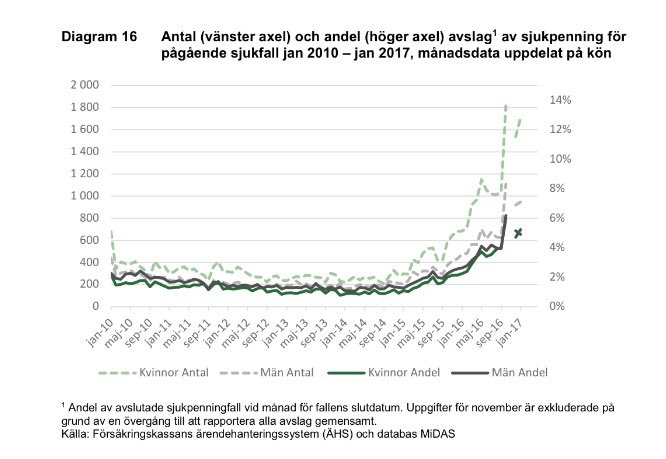
\includegraphics[width=\textwidth,height=\textheight,keepaspectratio]{diagram16.jpg}}]{12 okt 2017}{FK nekar allt oftare sjukpenning mitt i ett pågående sjukfall. Här ser vi närmast en explosionsartad utveckling.}{https://twitter.com/KjellRautio/status/918404541233627136}

\entry{13 okt 2017 - Barnhem byggs åter för funktionshindrade}{Maria Persdotter som är ordförande för RBU, Riksförbundet för Rörelsehindrade Barn och Ungdomar (RBU) skriver på Facebook:

\begin{quotation}\say{Ännu en kommun bygger nu barnboende. Inte den första, och det lär inte vara den sista heller. Det är detta som händer när familjer med barn med omfattande funktionsnedsättningar inte får/får behålla personliga assistans till barnet. 50-talet är på väg tillbaka med stormsteg.}\end{quotation}}{https://www.aftonbladet.se/ledare/a/L88kV/barnhem-byggs-ater-for-funktionshindrade}

\entry{13 okt 2017 - JAG DEMONSTRERAR FÖR EN MÄNSKLIG SJUKFÖRSÄKRING!}{Jag vågar för jag har genom mina 8 sjukärenden de senaste 21 månaderna sett att läkarintygens innehåll spelar ingen roll om handläggaren inte innehar viljan att ens försöka läsa och/eller förstå dem. Oavsett antalet ev kompletteringar. Fakta är inte viktigt för FKs bedömningar. Sjuktal är viktigt för FK.

Jag har blivit bedömd av 3st FMR-läkare på FK. Ingen har kunskap om ME/CFS men sätter sig ändå över mina behandlande läkare och specialister.
Någon kommunikation har FK inte velat ha med mig. När jag mailat handläggaren fakta, frågor och krav på svar på de fantasifulla motiveringarna till avslag, så har enhetschefen postat maktfullkomliga brev till mig 10-14 dagar senare. Dessa ”svar” har inte gett mig behövlig information och alltså har jag upprepade gånger nekats min rättssäkerhet - en grundläggande rättighet.

Jag har anklagats för att hitta på. Mina ord om min tillvaro har inte bedömts av FK som bevis eller sanningsenliga. Inte heller alla de tester jag gjort. Jag anklagas för att kunna hitta på. Men ingen - jag upprepar Ingen - väljer att må så här dåligt!

Ovanstående blir extra intressant när FK vägrar ge mig bevis för att de verkligen läst mina intyg o utredningar. De vägrar. Hur vet jag då att de inte hittar på? Hur vet jag att de inte fuskat och faktiskt lst intygen och förstått samt utrett/undersökt om det är något de inte fattat - innan de avslagit. Det är nämligen deras skyldighet. Varför anser de att deras ord duger som bevis, men inte mina?

Jag har i mina åtta ärenden stridit, via jurist, i FKs Omprövnad (OMP), jag har fått rätt retroaktivt i 4 ärenden ENDAST pga att det sista godkändes! Inte för att faktan ändrades i de ärendena. Jag har just nu 3 ärenden i Kammarrätten. Dessa ärenden baseras på samma oförmåga till arbete, men belastar nu rätten.}{\detokenize{https://www.facebook.com/photo.php?fbid=10213548199767055&set=a.1726167201702.95453.1464075288&type=3}}

\entry{14 okt 2017 - JAG DEMONSTRERAR FÖR EN MÄNSKLIGARE FÖRSÄKRINGSKASSA!}{För några veckor sedan kom besked från Försäkringskassan om att de inte helt överraskande (men ändå lika obegripligt) också överväger att avslå min nya ansökan om sjukpenning.}{\detokenize{https://www.facebook.com/photo.php?fbid=1569224069806420&set=a.162633263798848.39808.100001565259806&type=3}}


\entry{15 okt 2017 - Demonstration mot Forsäkringskassans hårdare bedömningar}{Hundratals människors samlades i Stockholm för att demonstrera mot Försäkringskassans allt hårdare bedömningar.}{http://www.tv4.se/nyheterna/klipp/demonstration-mot-fors%C3%A4kringskassans-h%C3%A5rdare-bed%C3%B6mningar-3939691}

\entry{16 okt. 2017}{Facktisdag igen och dags att ta hand om svinnet efter regeringens styrning av Försäkringskassan. Ni är lortar, ministrar. Ni äcklar mig.
Människor som slitit och betalat skatt i hela sitt liv. Plötsligt ställs de utan ersättning för att de inte blev friska på ett halvår.
Liv förstörs framför mina ögon samtidigt som regering och kommun använder de här människorna för att bevisa minskad sjukskrivningskostnad.
Regeringen. Ni är mobbaren på skolgården som i ens stunden slänger sand i ögonen på den svage i klasen och i andra säger \say{jag gjorde inget}.}{https://twitter.com/Skolinkvisition/status/920144374457085953}

\entry{16 okt. 2017 - \say{Rätt försäkring till rätt person}}{Detta är nog det mest kränkande denna myndighet faktiskt kan säga.
Är jag fel person?
Hur då?
Jag var rätt person under 6(!) år utan tvekan från FK. Sen förvandlades jag hux flux till fel person, utan någon förändring skett hos mig.}{https://twitter.com/livetsbilder/status/919982258857152512}

\entry{16 okt 2017}{Enda familj på plats förutom maken var min ALS-sjuke bror som höll tal. Han är snart 63 år, nekas sjukpenning och FK vill han arbetstränar.}{https://twitter.com/cwellton/status/919910166191071232}

\entry{16 okt 2017}{Jag misstänker att många av oss inser när vi ser ordet rättssäker och FK i samma mening så blir vi heligt förbannade. För de synkar inte.}{https://twitter.com/jag_e_pippi/status/919967834133889024}

\entry{16 oktober, 2017}{Försäkringskassan slår sig stolt för bröstet och tar credit för att sjuktalen sjunker. Men i deras statistik ingår inte alla vi som fått avslag på våra ansökningar om sjukpenning och blivit utförsäkrade. Vi är fortfarande sjuka och fortfarande sjukskrivna – ofta av flera läkare, men vi har ingen försörjning.}{https://newsaboutdisease.com/2017/10/16/samhallet-vill-inte-hjalpa-mig/}

\entry{17 okt 2017 - Sjuka blir fattiga av Strandhälls politik}{Antalet överprövningar ökade med 500 procent. Det här handlar inte om ett enskilt cancerfall, det handlar inte om en grupp rättshaverister.
Det handlar om många människor som förlorar sin trygghet när de som bäst behöver den. Både LO-förbund och TCO-förbund kritiserar hur deras medlemmar behandlas och visst är det galet när lärare uppmanas att söka andra jobb.}{https://www.aftonbladet.se/a/EdgWj}





\entry{17 okt 2017}{Så här beskrev en ombudsman ett medlemsärende och hur försäkringskassans tolkning av hårdare regler ska tillämpas: \begin{quotation}Pratade med en medlem i dag lärare hen har varit sjukskriven i 6 mån (utmattning) och med arbetsgivarens hjälp/ anpassningar lyckats komma upp i arbete till 75\% och en rehabplan som siktar på 100\%. \ldots Vet ni vad F.K säger, eftersom du kan arbeta i ett anpassat ARB, så kan du gå upp i 100\% i ett \say{enklare vanligt förekommande arbete på arbetsmarknaden}\end{quotation}}{https://twitter.com/cyrran/status/920500569424433152}





\entry{18 oktober 2017}{Regeringen måste se över de regelverk som styr Försäkringskassans arbete. \say{Det är oacceptabelt att människor får lida}, säger läkaren Lars G Wallander.}{http://www.barometern.se/kalmar/forsakringskassan-maste-lita-pa-lakarna/}

\entry{18 oktober 2017}{Är det dags att söka psykakuten när man öppnar ett avslag från Kammarrätten och skrattar hysteriskt samtidigt som kroppen krampar?}{https://twitter.com/jag_e_pippi/status/920639725949595650}



\entry{19 okt 2017 - L: Nu KU-anmäler vi Regnér för LSS-krisen}{För många barn och vuxna är assistansen skillnaden mellan ett liv i isolering och ett liv där varje människa kan leva så självständigt som möjligt. LSS-reformen är den största frihetsreform som genomförts i vårt land i modern tid.}{https://www.aftonbladet.se/debatt/a/zRLMb/l-nu-ku-anmaler-vi-regner-for-lss-krisen}

\entry{19 okt 2017 - Liberalerna KU-anmäler Regnér för LSS-brev}{Riksdagsledamoten Bengt Eliasson (L) KU-anmäler barn-, äldre- och jämställdhetsminister Åsa Regnér (S) för det direktiv hon gav Försäkringskassan om rätten till assistans, som även påverkade dem som omfattas av lagen om stöd och service till funktionshindrade (LSS).}{https://www.svd.se/liberalerna-ku-anmaler-regner-for-lss-brev}


\entry{19 okt 2017 - Hur kan sjuka få höra att de inte är sjuka?}{Systemet innebär också att handläggare utan medicinsk utbildning, som ibland inte ens träffat den sjuka personen, avgör om personen har arbetsförmåga eller inte. Detta trots att personen i fråga redan har läkarintyg från sjukvårdens läkare. Ibland kallas en försäkringsläkare in och avgör om du är sjuk eller inte trots att ni inte ens har träffats.

Tänk dig själv kränkningen i att någon du aldrig har träffat med bestämdhet hävdar att du inte är sjuk när du är så sjuk att du absolut inte orkar ta dig till jobbet eller ens tänka på det.}{https://www.aftonbladet.se/debatt/a/9jj0r/hur-kan-sjuka-fa-hora-att-de-inte-ar-sjuka}


\entry{20 okt 2017}{Vi behöver prata om att sjuka människor inte kan ha ett liv pga risk för indragen sjukpenning/ersättning. För att \say{det visar arbetsförmåga}.

Sjuka som inte kan arbeta borde uppmuntras att fylla livet med meningsfulla aktiviteter i stället för att hotas av indragen sjukpenning.
Jag hör ofta om medsjuka som är oroliga för \say{vad man får göra} utan att riskera att bli klassad som arbetsför. Den oron är helt befogad.

Jag hör om läkare säga att alla typer av aktivitet räknas om till arbetsförmåga idag, på ett helt orimligt sätt.

Jag har vänner som fått minskad sjukskrivning med motivering att de klarar att göra frukost eller åka kollektivt.

Människor undrar om de får skriva om sin situation, vara kreativa, gå ut i naturen, visa livsglädje, protestera, demonstrera.
Allt kan vändas till att arbetsförmåga finns trots att detta är ett helt orealistiskt resonemang.

Till och med att människor försöker argumentera för sin sak i processen mot FK kan användas som ett bevis på arbetsförmåga.

Som arbetsterapeut blir jag bedrövad av att människor berövas möjligh att leva ett meningsfullt liv trots sjukdom \& nedsatt arbetsförmåga.
Jag är less på att sjuka misstänkliggörs och att de som bedömer arbetsförmåga saknar grundläggande kunskap om hur människan fungerar.

Inte ens att någon klarar av att arbeta heltid en hel vecka är ett bevis på att den personen har 100\% arbetsförmåga året runt!

Att en människa som får nekad sjukpenning återgår i arbete en period är inte heller ett bevis på att FK tagit rätt beslut.
Personen kanske håller näsan över vattenytan en stund men sedan rasar ännu djupare ner i sjukdom! Kanske mister arbetsförmågan helt.

När vi vabbar barn försöker vi uppmuntra till sådant som är roligt de stunder det går. För att göra det uthärdligare att vara sjuk.
Men vi ser ju att trots att barnet har roligt är det för sjukt för normal aktivitetsnivå. Det finns ingen motsättning i det.
När du är sjuk är det viktigt att hitta saker som ger mening, tröst och distraktion. Trots sjukdom. Trots att arbetsförmågan är nedsatt.

Att behöva vara rädd för att det som ger mening felaktigt ska bedömas som arbetsförmåga sätter sjuka människor i en fruktansvärd sits.
Livet blir begränsat i onödan, pga andras (läs FKs) okunniga och maktfullkomliga antagningar om vad arbetsförmåga egentligen innebär.

Att jag vill fortsätta leva ett meningsfullt liv trots min situation, att jag kan känna livsglädje trots svår sjukdom borde väl vara bra?
Är inte arbetsnedsättande sjukdom straff nog? Måste vi lägga till ständig rädsla och en urtrist och händelselös tillvaro till det?
Tro det eller ej men livet tar faktiskt inte slut även om arbetsförmågan aldrig återkommer! Även om samhället påstår det! Det är en myt!}
{https://twitter.com/livetsbilder/status/921396161948286977}


\entry{20 okt 2017 - Hopplöst att vara sjuk i ett sjukt system}{Det har gått över 180 dagar av min sjukskrivning. Efter 180 dagar måste du i princip vara frisk, oavsett sjukdom. För sjuktalen i samhället måste ner. Behandlande läkares sjukskrivningar underkänns av Försäkringskassan och regler som de själva bestämmer. De sätter sig alltså över en utbildad läkares kompetens.

\ldots

Hur kan vi tillåta att Försäkringskassan dömer ut en läkares utlåtande?

\ldots

Ska vi verkligen drabbas så fruktansvärt hårt, vi som redan är drabbade av smärtsamma sjukdomar? Vem hjälper oss?

Friskförklarad av Försäkringskassan, den nya vårdcentralen.}{http://www.bt.se/insandare/hopplost-att-vara-sjuk-i-ett-sjukt-system/}






\entry{21 oktober 2017}{Antalet avslag på ansökningar om sjukpenning eller sjukersättning slår i taket. Under 2016 fick nästan dubbelt så många sjuka personer avslag på sina ansökningar jämfört med år 2014. Jag möter människor som är totalt förtvivlade och i vissa fall kan ha fått sin ekonomi körd i botten på grund av hur Försäkringskassan hanterat deras ärende.}{https://natjuristerna.nu/faktabanken/gisslan-hos-forsakringskassan/}



\entry{23 oktober 2017 - Ohållbar press på sjuka att jobba}{Jag möter dagligen människor som gör allt för att komma tillbaka till ett arbete, som bollas mellan myndigheter – men som egentligen inte är friska nog att arbeta. Det är ohållbart, skriver Eva Sjögren, sius-konsulent Arbetsförmedlingen.}{https://arbetet.se/2017/10/23/ohallbar-press-pa-sjuka-att-jobba/}

\entry{24 oktober 2017}{Fler än en gång har det stått i tidningen om läkare som är frustrerade över att Försäkringskassan inte godtar deras läkarintyg som grund för att bevilja den sjukskrivne ersättning.}{http://www.barometern.se/insandare/forsakringskassan-ska-hjalpa-inte-stjalpa/}


\entry{24 oktober 2017 - Alla får inte sina mänskliga rättigheter uppfyllda}{Idag firar vi FN-dagen. Vi i Funktionsrätt Sverige deltar i arbetet med flera av FN:s konventioner och för vårt intressepolitiska arbete är FN:s konvention om rättigheter för personer med funktionsnedsättningar, Funktionsrättskonventionen, en självklar ledstjärna. Tyvärr måste det sägas att Sverige inte på långa vägar uppfyller rättigheterna i alla FN:s konventioner.

Redan 2014 fick Sverige kritik från FN när det gäller situationen för personer med funktionsnedsättning. Det gällde bland annat det långsamma arbetet med att säkerställa Funktionsrättskonventionen i svensk lag, men även kritik mot sjunkande resurser för personlig assistans.}{http://funktionsratt.se/blogg/blogginlagg-alla-far-inte-sina-manskliga-rattigheter-uppfyllda/}

\entry{25 oktober 2017}{Av allt att döma har Försäkringskassans strävan efter att uppnå regeringens mål (9,0 sjukpenningdagar år 2020) gått ut över de försäkrades ekonomiska trygghet och rättssäkerhet. Många är de varningsklockor som just nu ringer.}{http://loblog.lo.se/valfard/fokusera-pa-sjukfranvarons-orsaker-istallet-for-pa-sjukpenningtalet/}


\entry{25 oktober 2017 }{Så sjuktalen fortsätter att minska och försäkringskassan och socialförsäkringsministern slår sig för bröstet. Men vilka betalar för detta?
Jag är en av dem. Sjukskriven på 75\% i 2,5 år pga extrem trötthet, värk mm. Fick diagnos fibromyalgi efter 2 år efter otaliga utredningar.

\ldots

Försäkringskassan gav avslag på min sjukpenning samtidigt som jag skulle påbörja min rehabilitering på heltid.}{https://twitter.com/AnnaFlodellLind/status/923220696146341888}

\entry{26 okt 2017}{My. God. The comments on this. The sheer awfulness of this.

\begin{quotation}\say{\textbf{BBC News England‏}

A woman who took part in karate competitions while claiming disability benefits is jailed for 15 months http://bbc.in/2zIxHfE}
\end{quotation}

1. This headline is so disingenuous I want to scream. The \say{primary fraud} was that she didn't disclose living with a partner. But this headline implies that Disabled people shouldn't have hobbies and interests and enjoy their lives. And people who didn't read the article are totally for it, calling her \say{scum.} FUCK YOU ALL. You try living on Disability benefits. Anywhere. It's not easy or fair or just.

2. She was filmed \say{covertly} taking part in these activities. There are people out there who take such pleasure in ruining Disabled lives. If you're the kind of person who wants to hurt people getting things they don't deserve, GO AFTER CORPORATIONS. Anyone who felt satisfied after ruining that woman's life, like they did a good thing? Fuck. You. Being Disabled is hard. THE UN LITERALLY GOT INVOLVED BECAUSE OF HOW HARD THE UK MADE IT. Disabled people should be able to have relationships, get married, live with partners, etc., without losing supports.

3. This is a horrible thing. This is not a victory for anyone except the ableist trash who enjoy seeing Disabled lives ruined.

4. There is no way benefits fraud outweighs corporate tax fraud. Anywhere.

I just. If you're abled and you feel like there's a huge angry monster looking down on you with scorn right now, it's probably me.
FYI: Take a good hard look, bc THAT'S what benefits fraud looks like.

Benefits fraud is almost never an abled person pretending to be Disabled bc it's easier than working. (It isn't easier than working.)

Benefits fraud is Disabled ppl trying to live our lives against the will of a system that hates us w/o losing support we absolutely NEED.

Benefits fraud is being told to deserve help we must live within the tiniest box imaginable and daring to step outside that box.

This woman is going to jail for BEING MARRIED and not telling the government bc it would mean she couldn't afford to live period.
Like. Do you get how unjust that is?

\say{Benefits fraud} is how abled people punish us for daring to try and live like they do.}{https://twitter.com/EbThen/status/923667589259251712}

\entry{26 oktober 2017 - Stupstocken som blev till ättestupa}{Det spelar ingen roll om du har tio års sjukintyg sedan tidigare och helt uppenbart inte är arbetsför. Det enda som bedöms är formuleringarna i sjukintygen, skriver debattören Helen Björnfoth.}{https://orebro.etc.se/debatt/stupstocken-som-blev-till-attestupa}


\entry{27 oktober 2017}{Försäkringskassan varnar: Ny dom leder till att många kommer att beviljas färre assistanstimmar}{https://assistanskoll.se/20171027-Forsekringskassan-varnar-Ny-dom-leder-till-manga-kommer-beviljas-ferre-assistanstimmar.html}


\entry{28 oktober 2017}{Den senaste domen handlar om assistans vid transporter till fritidsaktiviteter. Den tolkar nu Fk som att ingen tid får ges mellan hjälpbehov.

Domen 2012 (som började användas efter Regeringens regleringsbrev till Försäkringskassan 2015) säger att personlig assistans vid bad inte är ett grundläggande behov. Det tolkar Försäkringskassan som att ingen egenvård är grundläggande behov, alltså inte andning, äta via sond osv.

Domen 2009 säger att finfördelning av segt kött inte är ett grundläggande behov. Det tolkar Fk som att ingen hjälp vid matsituationen är att tolka som grundläggande behov, förutom att föra gaffeln till munnen.}{\detokenize{https://m.facebook.com/story.php?story_fbid=1931681160192693&id=100000524824319&comment_id=1931705076856968&notif_t=story_reshare&notif_id=1509182789816839&ref=m_notif}}

\entry{29 oktober 2017}{Det händer att jag blir omåttligt trött på en del politikers totala brist på kunskap om, eller ignorans för, funkisars levnadsvillkor. Som t.ex när man pratar om vikten av utbildning för att minska den stora arbetslösheten bland funkisar. Jättebra plan! Men hey, politiker, ni kanske ska börja med att se över TILLGÄNGLIGHETEN till utbildning. Här finns oerhört många bottnar, men ta t.ex det här enkla:

Om du ska kunna gå den utbildning du vill gå kanske du måste flytta. Måste du flytta kanske du byter kommun. Byter du kommun kommer alla kommunala stödinsatser du kanske har för att få livet att fungera, som t.ex färdtjänst, hemtjänst, ledsagning eller assistans, att omprövas. Och bara för att en kommun har beviljat en stödinsats betyder inte det att en annan kommun kommer att göra samma bedömning. Således vet du inte innan du har flyttat om ditt liv kommer att fungera eller inte på din nya bostadsort och om det inte fungerar kan du inte gå utbildningen som du har kommit in på. Samma visa, givetvis, om du har fått jobb på annan ort. Och det här är bara EN tillgänglighetsaspekt.

Politiker: Sluta att få det att låta som att det är en så enkel match när det är ni som sätter upp hindren.}{https://twitter.com/Miss_Bildad/status/924680900461424640}

\entry{30 oktober 2017}{Ändå genuint impad av skamlösheten. En del av de goda statsfinanserna är så klart brutala nedskärningar inom assistans och sjukpenning. Som man dessutom vägrar diskutera. Den samtida socialdemokratins stora problem är att de saknar ideologi bortom dogmen om goda statsfinanser.

Och som jag skrivit tidigare: det är på fullt allvar nu; det är inga överdrifter. Stöd som är nödvändigt för att folk ska kunna leva sina liv dras just nu undan. Det byggs barnhem för ungar med funktionshinder, det kommer bli en standardlösning utan assistans. Det är varje anständig människas ansvar att agera och utkräva ansvar av en regering som utan riksdagsbeslut eller debatt driver detta.}{https://twitter.com/nklsaltrmrk/status/924983817269665792}

\entry{30 oktober 2017}{De senaste dagarna har mitt Facebookflöde fyllts av hjärtskärande desperata rop på hjälp från vänner som inte vet om de kommer kunna fullfölja sina studier, fortsätta arbeta, träna, träffa vänner, vara förälder, vän och partner – allt det som de flesta tar för givet. Tar för givet utan en gnagande oro för att Försäkringskassan och/eller Sveriges domstolar nästa gång det är dags för omprövning kanske inte alls tycker ska vara det givna längre. Vänner som uttrycker att de paralyseras av rädsla. Rädsla att friheten ska tas ifrån dem, rädsla för serviceboende istället för den egna bostaden. En okänd granne på andra sidan väggen, istället för maken bredvid i sängen.}{http://blogg.likaunika.org/land-ska-med-lag-byggas/}

\entry{30 oktober 2017}{jag förstår inte för mitt liv vad som håller på att hända med LSS-vården, och framförallt inte att det är Socialdemokraterna som är orsaken \ldots det finns inga tvivel om att min brukare behöver personlig assistans dygnet runt
hen klarar sig inte utan assistans. hur är det möjligt att de skulle kunna dra in den?
\say{Därför att till och med personer som behöver hjälp att andas har fått indragen assistans}}{https://twitter.com/fakejullan/status/924932227586232320}


\entry{Försäkringskassans svar om Iris, 1: Inte sjuk}{Ettåriga Iris behöver hjälp dygnet runt för att andas – men hamnar mellan stolarna.}{http://www.gp.se/nyheter/g%C3%B6teborg/os%C3%A4ker-situation-f%C3%B6r-iris-r%C3%A4tt-att-andas-1.4306964}

\entry{Wendela, 11, kan inte andas själv – Försäkringskassan drar in hjälpen}{Wendela Bergsten, 11, i Habo lider av ett livslångt syndrom som gör att hennes andning måste övervakas dygnet runt. Försäkringskassan beslu...}
{https://www.expressen.se/gt/wendela-11-kan-inte-andas-sjalv-assistansen-dras-in/}


\entry{30 oktober 2017 - Regeringen måste ta bladet från munnen när det gäller personlig assistans}{Det är svårt att föreställa sig att den nuvarande situationen gällande LSS-insatsen (Lagen om stöd och service till visa funktionshindrade) personlig assistans kan bli värre. Endast 14 procent av de som söker assistans idag får sin ansökan beviljad. I mitten på 90-talet var situationen den omvända. Bara i år har mer än 1000 personer förlorat sin assistans.}{https://www.mynewsdesk.com/se/funktionsratt/pressreleases/regeringen-maaste-ta-bladet-fraan-munnen-naer-det-gaeller-personlig-assistans-2238816}

\entry{31 oktober 2017 - Stupstocken i sjukförsäkringen blev ättestupa}{Socialdemokraterna lovade en humanare sjukförsäkring inför förra valet. Nu slår de sig för bröstet och skryter över att de minsann tagit bort \say{stupstocken}. Vad de talar betydligt tystare om är de direktiv de gett till FK om att minska sjuktalen! Att minska sjuktalen! Inget prat om att förbättra människors hälsa dock.

Vad detta i realiteten lett till är att många människor (ofta efter väldigt lång sjuktid) plötsligt och utan förvarning får sin sjukpenning indragen.

Detta helt utan något stöd, utan de förväntas helt plötsligt att stå till arbetsmarknadens förfogande till 100 procent. Klarar man inte detta tappar man sin sjukpenninggrundade inkomst (SGI) och är dömd till fattigdom om man inte på något mirakulöst sätt blir frisk och arbetsför av denna behandling!!
}{http://www.na.se/opinion/debatt/stupstocken-i-sjukforsakringen-blev-attestupa}

\entry{31 oktober 2017 - Den totala sjukfrånvaron ligger på en historiskt rekordlåg nivå}{Socialdemokraterna och fackföreningsrörelsen kritiserade tidigare gemensamt alliansens tidsgränser och varnade för att utsatta människor redan efter ett halvt års sjukskrivning riskerar att fattiggöras genom att de går miste om såväl sin sjukpenning som sin anställning. Ingen blir friskare av att bli fattig och den som drabbats av stressrelaterad ohälsa blir inte bättre av att pressas och stressas ekonomiskt. Vad vi behöver, istället för att fattiggöra människor, är rejäla satsningar på förebyggande arbete och rehabilitering.}{http://loblog.lo.se/valfard/den-totala-sjukfranvaron-ligger-pa-en-historiskt-rekordlag-niva/}

\entry{31 oktober 2017 - Försäkringskassans nya assistansregler en skandal}{\say{Den 30 oktober 2017 var en ödets dag. En sådan att minnas i framtida historieskrivningar. En när det blev brutalt tydligt, att det som en trott aldrig skulle kunna hända till slut gjorde det.} Det skriver Christine Bylund, doktorand i etnologi vid Umeå universitet apropå Försäkringskassans beslut om nya bedömningsregler vid behov av personlig assistans.}{https://feministisktperspektiv.se/2017/10/31/forsakringskassans-beslut-ar-en-skandal/}

\entry{31 oktober 2017 - Sofia Mirjamsdotter: När Försäkringskassan stjälper i stället för hjälper}{Sjukförsäkring. Smaka på det ordet. Är det inte vackert?
En försäkring för den som är sjuk.

En försäkran om att den som är sjuk inte ska behöva oroa sig för att inte kunna betala räkningarna.

En möjlighet att ta hand om sig när kroppen säger ifrån.

Ett löfte från staten om att den ska ta hand om en, när man inte klarar sig själv. Det som också kallas samhällskontrakt. Vi betalar skatt till det gemensamma, som sedan tar hand om dem som bäst behöver det.

Sedan en tid är det inte längre ett löfte. Den som blir sjuk måste utanpå själva sjukdomen också oroa sig för om läkarintyget ska godkännas av Försäkringskassan.}{http://www.st.nu/opinion/ledare/sofia-mirjamsdotter-nar-forsakringskassan-stjalper-i-stallet-for-hjalper}

\entry[{
\includegraphics[width=\textwidth,height=\textheight,keepaspectratio]{DNd2yLLW4AAke-R.jpg}}]{31 okt 2017}{Genom att sparka på oss som redan ligger får \#Regeringen \#Alliansen \#Försäkringskassan ner sjuktalen i statistiken. Ruttet!}{https://twitter.com/A_sick_world/status/925338895851622400}


\entry{1 nov 2017 - Löfvens hårda attityd mot funktionshindrade}{Stefan Löfven riskerar att bli den statsminister som lägger ner assistanshjälpen till funktionshindrade. Den röd-gröna regeringen har hittills visat en obegripligt hård attityd mot människor med funktionsnedsättningar.
Bara 14 procent av dem som söker assistans får i dag sin ansökan beviljad. I år har mer än 1000 personer förlorat sin assistans och situationen för de funktionsnedsatta kommer att bli ännu värre. Nu vädjar till och med Försäkringskassans chef Ann-Marie Begler till regeringen. I ett alarmerande brev förklarar hon att en ny dom i Högsta förvaltningsdomstolen kan få “svåröverskådliga konsekvenser”. Nästan hälften av de funktionsnedsatta kan förlora sin hjälp i livet. Det handlar om 6000 människor.
Hela idén om allas rätt till fullvärdiga liv håller på att haverera. För frågan är vad som finns kvar när Löfvens regering genomfört sina besparingsprogram. Hemtjänst för vuxna och institutioner för små barn?}{https://www.aftonbladet.se/ledare/a/VOLvd/lofvens-harda-attityd-mot-funktionshindrade}

\entry{1 nov 2017 - Sveriges funktionshinder-politik på väg att misslyckas, Forskare: Vi riskerar allvarlig kritik från FN}{Vi lever i ett otillgängligt samhälle. Allt fler människor försätts i utanförskap. Jag tror inte att Sverige kan lyckas med sin funktionshinderspolitik det närmaste decenniet, skriver Jörgen Lundälv, funktionshinderforskare.}{https://hejaolika.se/artikel/sveriges-funktionshinder-politik-pa-vag-att-misslyckas}

\entry{1 nov 2017 - En mänskligare försäkringskassa}{Tillsammans – friska, sjuka och funktionsnedsatta – måste vi göra vår Försäkringskassa mänsklig igen. En Försäkringskassa som inte slänger ut människor till fattigdom eller osjälvständighet på grund av hårdtolkningar av dombeslut och regleringsbrev.}{http://solrosuppropet.se/2017/11/en-manskligare-forsakringskassa/}

\entry{1 nov 2017 - Det här är inte värdigt ett välfärdsland}{Det pågår ett välfärdssvek mot alla dem som får sin personliga assistans indragen i regeringens intensiva kostnadsjakt inom LSS.

På 1950-talet placerades barn med funktionshinder på olika institutioner, den tiden vill vi inte ha tillbaka. Trots detta bygger i dag kommuner barnboenden till funktionsnedsatta som fått indragen assistansersättning eller nekar handikappanpassningar av bostäder.

Barn ska få bo hemma hos föräldrar och syskon eller i varje fall i familjemiljö. Inte på en dåtidens intuition. Detta är inte värdigt Sverige som välfärdsnation. Det är en skrämmande utveckling. I Sverige ska alla ha möjlighet att delta i samhället utifrån sina förutsättningar. Inte gömmas och glömmas.}{http://www.gd.se/opinion/debatt/det-har-ar-inte-vardigt-ett-valfardsland}


\entry{2 nov 2017}{Hur kunde vi ge FK handläggarna en sådan makt över människors liv o död? De har ingen som helst medicinsk kompetens}{https://twitter.com/1000goodangels/status/926055393356320768}

\entry{2 nov 2017 - Sjukförsäkringen, en trygghet i upplösning?}{Allt fler får avslag på sin ansökan om sjukpenning. Thomas Persson opererade handen och innan rehabiliteringen var över drog Försäkringskassan in hans sjukpenning. Reglerna är oförändrade men trots det får allt fler nej på sin ansökan om sjukpenning.}{http://sverigesradio.se/sida/avsnitt/973707?programid=4091}

\entry{2 nov 2017 - Nu får hela familjer sina liv förstörda}{Rekordmånga förlorar nu sin personliga assistans. Folk ringer till oss och gråter. Jag och tusentals med mig lever i skräck.
Förstår inte regeringen vansinnet i det som är på väg att ske? skriver Anders Westgerd.}{https://www.expressen.se/debatt/nu-far-hela-familjer-sina-liv-forstorda/}

\entry{2 nov 2017 - Assistansen hotas – \say{det här är ett krig för vårt människovärde}}{Efter en dom i somras står det nu klart att rätten för assistansersättning inte gäller när det kommer till det som kallas väntetid och beredskap. Det framkommer av en bedömning försäkringskassan gör. Domen kan leda till att flera tusen personer förlorar assistansersättning från staten – något som Försäkringskassan varnat regeringen för. För ryggmärgsskadade Annika Taesler och hennes son riskerar detta att bli förödande. Hör även Lars Ohly, tidigare partiledare, numera ordförande i Funktionsrätt Sverige.}{https://www.tv4play.se/program/link/3942370}


\entry{2 nov 2017}{Dags att vakna ur din Törnrosasömn nu @strandhall
Sjukförsäkringen är vidrig numera! Knappast mänsklig. Hör när Ruth bland annat berättar om hur förhållningssättet till sjukförsäkringen varierat genom åren.

På 50-talet ville man ha frisk arbetskraft.
Då fick folk bli friska innan de återgick till arbetet.
Man gör ju bättre jobb då...effektivare.

Nu - 2017 - har kunskapen gått bakåt.
Nu ser man rest-arbetskraft. Som ska utnyttjas till sista droppen.
Finns inga jobb för den droppen. Så det känns väldigt tydligt när man tänker efter - det vi hör idag om effektivisering mm handliar bara om sista droppen.

När Regeringen skriker om att sjukförsäkringen är för dyr handlar det om deras prioriteringar och vad de tror är effektivt - för stunden.
Regeringen glömmer att en droppe sakta urholkar stenen.
Regeringen urholkar den riktiga arbetskraften genom att låta sista droppen vinna.}{https://twitter.com/jag_e_pippi/status/926023064722210816}

\entry{2 nov 2017 - Att andas inget grundläggande behov}{Att andas räknas inte längre som ett grundläggande behov av försäkringskassan. Det säger en hel del om vilken absurd nivå lagtolkningarna redan nu ligger på gällande LSS.}{https://www.ottar.se/artiklar/att-andas-inget-grundl-ggande-behov}

\entry{2 nov 2017}{Skrämmande när staten sätter prislappar på människor. \#svpol \#försäkringskassan \#assistans}{https://twitter.com/block_lennart/status/926010356224417799}


\entry{3 nov 2017 - \say{Regnér - och Alliansen - har satt spiken i kistan för LSS}}{Fredagen den 27 oktober. Kanske kommer många att minnas den som en ödesdag. En dag när vi som samhälle valde väg, när vi accepterade att en grupp människor och medborgare inte skulle vara en del av oss andra. Att det, de, inte är värda det. En skammens dag.}{https://www.dagenssamhalle.se/debatt/regner-och-alliansen-har-satt-spiken-i-kistan-lss-19330}

\entry{3 nov 2017 - \say{Löntagare måste kunna lita på sjukförsäkringen}}{Fler hamnar i kläm när de får sjukpenningen indragen av Försäkringskassan. De som drabbats av sjukdom måste få ekonomisk trygghet och en rättssäker bedömning. Regeringen bör se över sin styrning av Försäkringskassan, skriver Torbjörn Johansson och Kjell Rautio, LO.}{https://www.svd.se/lontagare-maste-kunna-lita-pa-sjukforsakringen}

\entry{3 nov 2017 - Att förstöra ett liv}{\say{\say{Fruktar ni att fler kommer att välja att bli funktionshindrade om villkoren blir för humana?} vill man retoriskt fråga beslutsfattarna}, skriver Toivo Jokkala.}{https://www.arbetaren.se/2017/11/03/att-forstora-ett-liv/}

\entry{3 nov 2017}{Vi som haft turen att inte ha ett handikapp. Det är vår förbannade skyldighet att se till att de som inte haft samma tur har det så bra som de möjligen kan ha det! Och glöm aldrig att allt kan ändras på en minut. Ingen är säker, hur stark man än är!  \#Assistans  \#räddaLSS}{https://twitter.com/LOGavert/status/926560250832007168}

\entry{3 nov 2017}{Jag vill förtydliga en sak: Att bli nekad sjukpenning har flera dimensioner. Och det handlar om SÅ mycket mer än \say{bara} ekonomi!

Visst det innebär att min försörjning uteblir men det handlar också om att mina begränsningar förnekas.
Att påstå att jag kan arbeta i nuvarande skick är ett hån mot hur extremt begränsat min sjukdom tvingar mig att leva.
Att neka sjukpenning är samma sak som att säga att hela mitt begränsade liv är en lögn. Vem vill leva så och göra de val jag tvingas göra?

Genom att intyga mitt behov av sjukskrivning bekräftar läkaren att min situation är giltig och rimlig.
Försäkringskassan bekräftar eller förkastar sedan i sitt beslut vårdens bedömning.
När det senare sker - jag får avslag - underkänns på sätt och vis vårdens bekräftelse. Och min situation och mina behov ogiltigförklaras.

Hela samhällsapparaten tvingas nu se mig som frisk och fullt arbetsför trots att FK är enda instansen som säger att de ser mig så.
Dessutom går all tid nu och framöver att gå till detta - att försöka få sjukpenningen godkänd i rättslig process.
För min man tvingas dels arbeta ensam för hela familjens försörjning plus att han får alla kontakter relaterat till processen.

Min läkare är överbelastad så den tid jag har att ta i anspråk går även här enbart till rättsprocess och sjukpenning.
Mina andra eventuella behov av vård och stödåtgärder får sättas åt sidan. För ingen har varken tid eller ork att ta hand om detta också.

Vi kan inte skippa rättsprocessen, för vi klarar oss inte på lång sikt enbart på min mans lön. Därför måste den prioriteras först.
Även om de innebär att andra basala behov måste stå tillbaka. Att få avslag på sjukpenning påverkar mer än min inkomst, det gör sönder mig.
}{https://twitter.com/livetsbilder/status/926448341411647489}

\entry{4 nov 2017 - Hallå socialdemokrater, kan man få ett svar?}{Friheten för varje människa, att få bestämma över sitt eget liv och sin egen framtid är själva kärnan i liberalismen. Att ta strid mot de besparingar som nu genomförs och aviseras inom personlig assistans är att försvara friheten.}{http://www.gd.se/opinion/debatt/halla-socialdemokrater-kan-man-fa-ett-svar?referrer=app}{}

\entry{4 nov 2017 - Att andas räknas inte som ett grundläggande behov}{Men det var mycket jag inte riktigt förstod, som det där med att bo. Barnen jag lekte med var lika gamla som jag, några äldre med cp- eller neurosedynskador, några hade utvecklingstörningar. De flesta var på besök för behandling men en flicka åkte inte hem när vistelsen var slut. Hon levde på avdelningen på obestämd tid, utan möjligheten att växa upp med sin mamma och pappa.
Det var ofattbart. Hur kunde det vara så? Måste inte barn få vara med sina föräldrar?
\ldots
Men ett välfärdsland som tvingar föräldrar att lämna bort sina ungar för att kraften slutligen sinat, för att kärleken som underhållit år av nattvak och omsorg till slut drivit dem in i väggen, det är inget värdigt land.
}{https://www.expressen.se/kronikorer/jenny-stromstedt/att-andas-raknas-inte-som-ett-grundlaggande-behov/?social=twtr}

\entry{5 nov 2017 - Blev av med sin assistans – har skickats till akuten tre gånger}{Sen strokedrabbade Mikael Foss för sex veckor sedan blev av med delar av sin personliga assistans så har han fått uppsöka akuten tre gånger.}{\detokenize{http://sverigesradio.se/sida/artikel.aspx?programid=86&artikel=6813440}}

\entry{6 nov 2017 - STOPP! Tusentals människors liv slås sönder}{En samlad funktionshinderrörelse säger härmed stopp! Regeringen måste ta sitt ansvar och agera. Vi kräver en plan för en lagändring och för hur LSS intentioner ska återställas. I slutändan handlar det om vilket samhälle och människosyn vi vill ha i Sverige.}{https://www.dagenssamhalle.se/debatt/stopp-tusentals-manniskors-liv-slas-sonder-19338}

\entry{6 nov 2017 - Sofia Mirjamsdotter: Det finns pengar till sjukförsäkringen}{Allt fler människors liv rasar, inte endast på grund av sjukdom utan också pga en raserad ekonomi}{http://www.st.nu/opinion/ledare/sofia-mirjamsdotter-det-finns-pengar-till-sjukforsakringen}

\entry{6 nov 2017 - Hur ska jag förklara för min son att ni vill slita isär hans familj?}{\emph{Jag tänker att det bara inte får hända – i nästa sekund funderar jag på hur jag ska ta livet av mig om det drabbar mig.}

Så kom den då, i lördags kväll: panikångestattacken.
\ldots
Detta är att likställa med en brandman som bara får lön just när det larmar, eller en expedit som inte får betalt när butiken är tom.

För mig, som är totalförlamad, handlar det om att förutsäga att ”om 47 minuter måste jag schemalägga en assistent, så jag kan dricka”, eller ”om 1 timme, 34 minuter och 15 sekunder kommer jag få ett hostanfall som riskerar att kväva mig”.
}{https://www.svt.se/opinion/annika-taesler-om-lss}

\entry{6 nov 2017}{Tror du det är en tillfällighet att såväl läkare, granskande myndigheter, enskilda försäkrade och fackliga organisationer just nu larmar om att de sjukas ekonomiska trygghet och rättssäkerhet kommer på undantag när Försäkringskassan (FK) försöker uppnå sitt siffermål?}{http://www.nsd.se/nyheter/siffrornas-makt-over-bokstaverna-nm4682055.aspx}

\entry{6 nov 2017 - Läkare kritisk mot Försäkringskassans hantering}{Patienter som är förtvivlade över utebliven sjukpenning och växande frustration bland läkarna i takt med att antalet avslag från Försäkringskassan ökar}{\detokenize{http://sverigesradio.se/sida/artikel.aspx?programid=78&artikel=6814848}}

\entry{6 nov 2017 - Sjuka drabbas – tre gånger fler nekas sjukpenning}{Trots fem läkarintyg nekades dubbelt cancerdrabbade Anne-Christine Östman i Hallviken sjukpenning för sin utmattningsdepression.}{\detokenize{http://sverigesradio.se/sida/artikel.aspx?programid=78&artikel=6813616}}

\entry{6 nov 2017 - Thomas Bull, Justitieråd Högsta Förvaltningsdomstolen – \say{Vårt avgörande hade inte något med väntetid eller beredskap att göra}}{Thomas Bull menar alltså att Försäkringskassan gör tolkningar av frågor som HFD inte hade i uppdrag att bedöma i den aktuella domen. }{https://assistanskoll.se/20171106-Thomas-Bull-HFd-avgorande-inte-ventetid-beredskap-gora.html}

\entry{6 nov 2017 - Stress - måste vi leva med den?}{Psykisk ohälsa ökar. Stress ökar. Försäkringskassan har börjat neka fler personer rätten till sjukpenning, märkligt nog utifrån att regeringen gett dem i uppdrag att sänka sjuktalen\ldots}{https://www.lararforbundet.se/bloggar/lararforbundets-utredarblogg/stress-maaste-vi-leva-med-den}

\entry{6 nov 2017 - Mia Modig: LSS måste börja användas enligt lagens syften}{En nödstopp måste införas för den nedmontering av LSS som pågår. Försäkringskassan måste börja tillämpar LSS med tonvikt på lagens syften: att skapa goda levnadsvillkor, jämlikhet och självbestämmande.}{https://asikt.dn.se/asikt/debatt/lss-maste-borja-anvandas-enligt-lagens-syften/}


\entry{7 nov 2017}{\#vadfanfårjag Försäkringskassan redovisar minskade antal sjukskrivna. Undrar varför? Sjuk utan ersättning! \#försäkringskassan}{https://twitter.com/EijaMirjam/status/927950352095285248}

\entry{7 nov 2017 - Kroniskt sjuka borde inse vilken belastning de är för samhället}{Nu var många så fräcka att de dog i stället för att gå till jobbet. En del var än mer fräcka och tog livet av sig.}{http://www.st.nu/opinion/insandare/kroniskt-sjuka-borde-inse-vilken-belastning-de-ar-for-samhallet}

\entry{7 nov 2017}{Hade inte självmordstankar före jag förlorade min inkomst, trots giltiga intyg. Men hade troligen varit på väg tillbaka nu annars.}{https://twitter.com/Shadilly/status/927951684755652609}

\entry{7 nov 2017 - Lagändring på gång – MR-juristen Andrea Bondesson reder ut rättsläget}{I den rättsliga analysen betonar också Andrea Bondesson att Försäkringskassans tolkning står i strid med rättsstatens principer, men även bryter mot såväl Europakonventionen som Funktionsrättskonventionen. Dessutom står den i strid med de intentioner som framkommer i förarbeten till LSS.}{https://funktionsrattskonventionen.se/lagandring-pa-gang-mr-juristen-andrea-bondesson-utreder-rattslaget/}

\entry{7 nov 2017 - Janne från Sikås nekas sjukpenning: Man bryter ihop}{Läkarna är jätteupprörda, de tycker man ska dra det här inför Europadomstolen så att Sverige får skämmas}{\detokenize{http://sverigesradio.se/sida/artikel.aspx?programid=78&artikel=6815441}}

\entry{7 nov 2017 - \say{Sjukskrivna hänvisas till jobb för pigga, glada och alerta}}{Bedömning av arbetsförmåga och tillämpning av sjukförsäkringen måste verklighetsförankras och hänsyn måste tas till människors faktiska förmåga att kunna försörja sig på arbetsmarknaden.}{https://www.arbetsvarlden.se/kronikor/sjukskrivna-hanvisas-till-jobb-dar-man-ska-vara-glad-pigg-och-alert/}

\entry{7 nov 2017}{En människa av idag röstar bara på @socialdemokrat fram till dess att den själv eller nära anhörig kommer i kontakt med \#försäkringskassan}{https://twitter.com/Naturstacken/status/927950188488126464}

\entry{7 nov 2017}{Hej Annika

För många lärare som drabbats av utmattning vänder livet just nu. Från lön till avslag på sjukpenning. Du bär faktiskt ansvaret. När du blev minister tänkte jag \say{äntligen någon som förstår}. Nu, efter tre år av rödgrön regering, tänker jag \say{hur kunde det gå så snett.} Visst. Det är mest low lifes som jag som klagar. Sjukförsäkringen är säkert ingen fråga som får så mycket uppmärksamhet på mingel.
Men om knappt ett år är det val. Den där gången på året då plötsligt alla människor är lika mycket värda. Vi får se hur det går för dig då.
För varje person Försäkringskassan utförsäkrar, som konsekvens av ditt niodagarsmål, finns ett gäng nära släkt och vänner med rösträtt.
Jag kommer att göra mitt för att så många som möjligt ska förstå att det är du och dina kollegor i regeringen som bär ansvaret.
En röst på Socialdemokraterna eller Miljöpartiet är en röst för ett välfärdssamhälle som INTE finns där för alla när livet vänder. }{https://twitter.com/Skolinkvisition/status/927947095302131712}

\entry{7 nov 2017 - Åsa Regnér (S) ger falsk bild av assistanshaveriet}{Under denna tid har mer än tusen personer förlorat sin assistans, och 80-90 procent av alla som ansöker får avslag.

Detta beror inte på att människor med svåra funktionshinder, som under lång tid haft assistans, nu kan klara sig utan denna. Inte heller är de fuskare eller lurar staten på pengar.

Detta beror på en socialdemokratisk regering som, enligt den förra socialministern Ingela Thalén (S), ”förlorat sin ideologiska kompass” och ”nu är ett parti som värnat utsatta grupper på väg att skjuta LSS i sank”. Det skrev Thalén för ett år sedan.

\ldots

Försäkringskassan brydde sig aldrig om dessa domar i HFD fram till hösten 2015, då två av domarna redan funnits i flera år. Men då förklarade finansminister Magdalena Andersson (S) att vi måste spara på assistansersättning och sjukförsäkring för att ha råd med flyktingmottagningen.

\ldots

Väck misstroendeförklaring mot Åsa Regnér i riksdagen. Hon har avsiktligt misstolkat förarbetena i lagstiftningen och försatt en grupp hon är satt att värna i en utsatt och farlig situation. Det är skäl nog för riksdagen att agera.}{http://www.gp.se/nyheter/debatt/%C3%A5sa-regn%C3%A9r-s-ger-falsk-bild-av-assistanshaveriet-1.4807839}

\entry{8 nov 2017 - Domare: Försäkringskassan har övertolkat domen}{Försäkringskassan kan i teorin backa från sitt beslut om hur man tolkat domen – men det kommer inte att ske.}{https://www.svd.se/domare-forsakringskassan-har-tolkat-domen-fel}


\entry{8 nov 2017 - \say{Sjuka ska ha rätt att vara sjukskrivna}}{När allt fler får avslag på sin sjukpenning menar distriktsläkare Margaretha Lööf-Johansson från Brunflo, att det måste till en förändring från politikerna.

– Detta är inte rätt att sjuka människor ska behöva hamna i en sån här situation, säger Margaretha Lööf-Johansson, medicinskt ansvarig läkare i Brunflo.

Hon menar också att rätten att bli sjukskriven när man är sjuk är en självklar del av välfärden.}{\detokenize{http://sverigesradio.se/sida/artikel.aspx?programid=78&artikel=6816507}}

\entry{8 nov 2017 - En introduktion till assistanskrisen - Niklas Altermark, Fil. Dr.
Statsvetenskapliga institutionen
Lunds Universitet}{Sett ur ett demokratiperspektiv är det problematiskt att så genomgripande förändringar av en
central socialpolitisk insats kan ske utan lagändringar och möjlighet till ansvarsutkrävande.}{https://niklasaltermark.files.wordpress.com/2017/11/assistanskrisen2_altermark2.pdf}

\entry{8 nov 2017 - Försäkringskassan övertolkar assistansdom}{Försäkringskassan gör en långtgående tolkning av rätten till personlig assistans i den nya domen från Högsta förvaltningsdomstolen. Det menar justitierådet Thomas Bull i Högsta förvaltningsdomstolen, som själv varit med och dömt.}{\detokenize{http://sverigesradio.se/sida/artikel.aspx?programid=83&artikel=6815940}}


\entry{8 nov 2017 - Socialutskottet kräver nytt möte med Försäkringskassan}{Försäkringskassans chef Ann-Marie Begler kallas åter till riksdagens socialutskott för att förklara kassans hantering av assistansersättning till funktionshindrade.

Orsaken är att justitierådet i Högsta förvaltningsdomstolen har dömt ut Försäkringskassans tolkning av domen om hur assistansersättning ska betalas ut.}{\detokenize{http://sverigesradio.se/sida/artikel.aspx?programid=83&artikel=6816273&utm_source=dlvr.it&utm_medium=twitter}}

\entry{8 nov 2017 - En trygghet i upplösning??}{Jag vrider mig av obehag bara av att läsa det hon säger, men vad är det då som jag reagerar så kraftigt på?}{https://livetsbilder.blogspot.se/2017/11/en-trygghet-i-upplosning.html?m=1}

\entry{8 nov 2017}{Försäkringskassans förnekande av min verklighet och deras officiella hållning kring sjukpenningtalen samt regeringens \say{här finns inget att diskutera} - attityd skadar mig och så många andra.

Deras mantran om \say{rätt ersättning till rätt person} och om att \say{de flesta får sin sjukpenning godkänd} antyder att jag är fel person och att de tagit rätt beslut.

Deras mantra om att \say{ökade avslag beror på ökad kvalitet på bedömningarna} antyder att mina 6 år med godkänd sjukskrivning var ett misstag.}{https://twitter.com/livetsbilder/status/928338716426473478}

\entry{8 nov 2017}{Den 27 november går mitt nuvarande sjukintyg ut. Återigen innebär det den där osäkerheten om Försäkringskassan kommer att godkänna det nya som kommer.
Detta trots att jag det senaste året varit inlagd på psykiatrins slutenvård tre gånger för suicidprevention.}{https://twitter.com/pippiglassbil/status/928169796834938880}

\entry{8 nov 2017 - Stor ökning av barn som förlorar personlig assistans}{Under årets första sex månader förlorade nästan dubbelt så många barn den statliga ersättningen för personlig assistans som under samma period förra året.}{https://www.dn.se/nyheter/politik/stor-okning-av-barn-som-forlorar-personlig-assistans/}

\entry{8 nov 2017 - Sjuka i kläm när de \say{bollas} över till Arbetsförmedlingen}{Vissa är för friska för att få pengar från Försäkringskassan men för sjuka för att få hjälp från Arbetsförmedlingen. Sjuka kommer i kläm mellan myndigheterna.}{\detokenize{http://sverigesradio.se/sida/artikel.aspx?programid=78&artikel=6815988}}

\entry{8 nov 2017}{Jag är less på att mitt liv reduceras till \say{upplevelser} som ifrågasätts. Att mina ord om min situation är mindre giltiga för att de är mina! \#fkstress}{https://twitter.com/livetsbilder/status/928530898835951616}

\entry{8 nov 2017 - Försäkringskassan och Regnér skyller ifrån sig}{Försäkringskassan drar långtgående slutsatser om rätten till assistansersättning baserat på ett antal domar från Högsta Förvaltningsdomstolen.  I flera fall om åtgärder som inte ens ingått i rättens bedömning. Som ett resultat slås människors och familjers livs i spillror, men de ansvariga skyller ifrån sig.}{https://www.dagenssamhalle.se/debatt/forsakringskassan-och-regner-skyller-ifran-sig-19407}

\entry{8 nov 2017}{Krocken mellan Försäkringskassans bedömning av min situation - och hur mitt liv faktiskt ser ut - är brutal. Det tär på mig och min självkänsla.
Maktobalansen i vårt förhållande är total. De har all makt och jag har ingen. Mina ord betyder ingenting i sammanhanget - men mina ord är allt jag har.
Trots att jag vet att min verklighet är sann - får deras tvivel mig att tvivla på mig själv. På min kompetens som finns där trots att kapaciteten brister - och på om kapaciteten verkligen brister så mycket som jag påstår.

Det får mig i dåliga stunder att undra om det kanske faktiskt är min verklighetsförankring som är dålig - inte politikernas och Försäkringskassans.
Men jag vet ju att om jag inte mått så här dåligt på riktigt hade jag aldrig hamnat här. Jag hade aldrig stannat kvar i den här förnedrande positionen.
Men trots att jag vet så tvivlar jag. På min förmåga att analysera situationen. Om mina texter är relevanta eller bara rättshaveristiskt svammel.

Det är läskigt, och gör mig rädd - men mest gör det mig ARG!

Försäkringskassans förnekande av min verklighet och deras officiella hållning kring sjukpenningtalen samt regeringens \say{här finns inget att diskutera} - attityd skadar mig och så många andra. Deras mantran om \say{rätt ersättning till rätt person} och om att \say{de flesta får sin sjukpenning godkänd} antyder att jag är fel person och att de tagit rätt beslut.

Deras mantra om attt \say{ökade avslag beror på ökad kvalitet på bedömningarna} antyder att mina 6 år med godkänd sjukskrivning var ett misstag.

Hur ska jag annars tolka det? Hur ska jag tolka deras brist på förståelse på min och så många andras situation. Deras totala sågning av läkarnas intyg. Högre kvalitet?
}{https://twitter.com/livetsbilder/status/928338716426473478}

\entry{9 nov 2017 - Natasha har blivit av med sin personliga assistent}{Skånskan träffar Peter Wallström på hans läkarexpedition för att prata om Försäkringskassans beslut.
– Det första jag tänkte var \say{Varför i h-e? Är de inte kloka?}, säger Peter Wallström.}{http://www.skd.se/2017/11/09/natasha-har-blivit-av-med-sin-personliga-assistent/}

\entry{9 nov 2017}{Bästa Stefan Löfven jag höll på att mista mitt hem när jag blev utförsäkrad av Försäkringskassan. Hur går det nästa gång? Blir jag hemlös?}{https://twitter.com/UllaBNilsson/status/928612049218883584}

\entry{9 nov 2017 - Eva Nordqvist, rättschef, Försäkringskassan – ”Vi har inte anledning att ändra vårt rättsliga ställningstagande”}{Trots att justitierådet Thomas Bull i HFD sagt att deras dom inte sade något om väntetid eller beredskap ändrar inte Försäkringskassan sitt ställningstagande.}{https://assistanskoll.se/20171109-Nordqvist-Forsekringskassan-inte-endra-stellningstagande.html}


\entry{9 nov 2017}{Japp. Normavvikande människor måste förvandlas till mätbara objekt för att åtnjuta samma rättigheter som normfungerande människor.}{https://twitter.com/Jonna_A/status/928560677379346432}

\entry{9 nov 2017}{S gick till val på trygghet för sjuka och skadade.  @strandhall har med sitt regleringsbrev krackelerat den strimma av trygghet som fanns. Nu balanserar alla sjuka på slak lina...}{https://twitter.com/UllaBNilsson/status/928652685980692485}
\entry{9 nov 2017 - Många vittnar om att de far illa av skärpt bedömning för sjukpenning}{Hårdare regler för sjukpenning ställer många människor i en svår situation.}{\detokenize{http://sverigesradio.se/sida/artikel.aspx?programid=78&artikel=6818077}}

\entry{9 nov 2017}{Bli kung på \#Försäkringskassan verkar enkelt. Man behöver bara tolka domslut som inte handlar om det man jobbar med och sedan med hänvisning till detta säga nej till allt.  Lättast om man ändå skiter i såväl förord som domar}{https://twitter.com/mickeastrom/status/928801816896266240}

\entry{9 nov 2017 - Larmar till FN om assistanskrisen}{Det här är också en utveckling som inte bara gäller personlig assistans. Vi upplever att rättigheter får allt mindre betydelse och att de allt oftare filtreras genom finansdepartementet. Det ser vi inom många områden, säger Rasmus Isaksson.}{http://funktionshinderpolitik.se/larmar-till-fn-om-assistanskrisen/}

\entry{10 nov 2017 - Skärp er, det handlar om svårt sjuka barn}{Man kan tro att djävulens verkliga advokater tagit över assistansersättningen till funktionshindrade. Kanske har de flyttat in på Försäkringskassan som just nu hotar att ta assistansen från ytterligare 6000 människor med funktionsnedsättningar.

Det handlar om barn med svåra funktionshinder. Det handlar om vuxna som kanske inte längre kan komma till jobbet. Om människor som byggt upp sina liv med hjälp av assistenter, men som nu riskerar att förlora allt.}{https://www.aftonbladet.se/ledare/a/kqnWX/skarp-er-det-handlar-om-svart-sjuka-barn}

\entry{10 nov 2017}{\say{Bromsa sjukskrivningskostnaderna} är något helt annat än att minska ohälsan!}{https://twitter.com/ylva_engstrom/status/928925216583180290}

\entry{10 nov 2017 - Forskare: Försäkringskassan vantolkar LSS konsekvent}{Många av Försäkringskassans nekande beslut om personlig assistans efter en uppmärksammad dom i somras strider mot lagen. I stället för att följa LSS tar myndigheten rygg på sina egna vägledningsdokument.
– Försäkringskassan ger sig rätten att fritt välja vad i domen de vill följa, säger Lennart Erlandsson, filosofie doktor och lektor i juridik vid Högskolan Kristianstad.}{https://feministisktperspektiv.se/2017/11/10/expert-forsakringskassans-styrdokument-strider-mot-lss/}

\entry{10 nov 2017 - Vi hjälper DN-reporter med fördjupande fakta om sjukskrivningar}{Vad är det som varit tufft och för vem har det varit tufft? Vi vet tyvärr svaren på de två frågorna. Det tuffa har varit att ge Försäkringskassan i uppdrag att minska antalet sjukdagar till 9 dagar/person och år. Det tuffa har varit att inte ge vika när pressen fyllts med vittnesskildringar från sjuka som har fått avslag på sin ansökan om sjukpenning. Det tuffa har varit att inte svara på frågor om hur individer har drabbats. Det tuffa har varit att styra bort diskussionen från det faktum att nedskärningarna i välfärden fortsatt och att den avsiktsförklaring som kommuner och landsting lovat ministern ska lösa problemen inte fungerar (läs tex om hur Göteborg stad inte hanterar ökad arbetsbelastning). Att folk inte bivit friskare utan att de bara plötsligt blivit utan ersättning och därmed inte längre finns med som sjuka i statistiken över sjuktal. Det är de sjuka som det varit tufft för.}{http://tankesmedjanbalans.se/vi-hjalper-dn-reporter-med-fordjupande-fakta-om-sjukskrivningar/}

\entry{10 nov 2017}{Så här är det: Vid en del vanliga funktionsnedsättningar så krävs det mycket förutsägbarhet för att vi inte ska göras illa bara av att existera. Nej, vi växer inte ifrån det. Nej, det är inte moralsikt sämre att funka så.}{https://twitter.com/Jonna_A/status/929297299423064064}


\entry{11 nov 2017}{Läser precis artikeln i DN. \say{Vänt utvecklingen med sjukskrivningskostnaderna}. Iskall omskrivning för ökad utslagning av långtidssjuka. Och du är stolt över det?}{https://twitter.com/TornbergHakan/status/929276598599155712}

\entry{11 nov 2017}{Skulle vilja veta hur @dagensnyheter tänker när man inte tar upp vad som gömmer sig bakom det fina \say{lyckats sänka sjuktalen}? För sanningen är att sjuka människor står utan försörjning enkom pga detta mål.}{https://twitter.com/pippiglassbil/status/929316520597114881}


\entry{11 nov 2017 - Brevet från Försäkringskassan kan trasa sönder Peters värld}{Enligt de nya regler som Försäkringskassan börjat tillämpa, baserat på en dom i Högsta förvaltningsrätten, ger väntetid ingen lön alls. Då går det inte att rekrytera personal. - Det är som om kassörskan i mataffären bara skulle få betalt när det är varor på bandet, säger Bo Gunnar.}{https://www.dn.se/nyheter/sverige/brevet-fran-forsakringskassan-kan-trasa-sonder-peters-varld}

\entry{11 nov 2017 - Funkisförälder: "Väntan på det fruktade brevet från Försäkringskassan – ska det behöva vara så..?}{Är det verkligen värdigt Sverige att individer och deras anhöriga ska känna en oro över sin tillvaro och inte känna att man har möjlighet att påverka sin egen situation?

• Att tvingas bli utelämnad till oförstående tjänstemän och politiker?

• Att tvingas att anpassa sitt eget liv till någon annans schema och agenda?

• Att inte längre kunna få göra det man vill, när man vill (till exempel så självklara saker som en promenad, handla eller träffa vänner)?}{http://www.allehanda.se/opinion/insandare/funkisforalder-vantan-pa-det-fruktade-brevet-fran-forsakringskassan-ska-det-behova-vara-sa}

\entry{12 nov 2017 - Läsartext: Min storebror har grundläggande behov precis som vem som helst}{Just detta har från ett tidigt skede i mitt liv känts så himla orättvist. Varför ska mina föräldrar och min storebror behöva ”straffas” för att han som individ föddes med en svår cp-skada?
För mig som syskon är det absolut inte okej att olika delar av samhället pratar över huvudet på honom om hur stor kostnad han är för samhället. Min storebror älskar sport, musik, mat, kramar och godis. Speciellt dansbandsmusik, olika måltider som min pappa lagar samt geléråttor. Han är en individ och inte enbart en siffra bland all statistik.}{\detokenize{https://www.sydsvenskan.se/2017-11-13/min-storebror-har-grundlaggande-behov-precis-som-vem-som-helst?utm_source=tw&utm_term=21e17928-d735-5e38-82d6-9aafeed0fcb4&utm_medium=list-bottom&utm_campaign=ushares}}


\entry{12 nov 2017}{Om Franz Kafka nånsin känner för att uppstiga ur graven och skriva en uppföljare till \say{Processen} kanske han kan skriva om hur det är att vara sjuk i sverige.}{https://twitter.com/Snufkin89/status/929687068741160961}

\entry{12 nov 2017}{Jag är det svarta fåret. Inte i familjen. I Sverige. Jag är den ingen vill ha. Den ingen vill betala skatt för. Den ingen vill se. Den ingen behöver. Sjuk. \#utförsäkrad fattigjord och olönsam. Paria.}{https://twitter.com/CatzSto/status/929822225754148865}

\entry{12 nov 2017 - Jenny Wennberg: Assistanshaveriet är regeringens verk}{Åsa Regnér är ansvarigt statsråd. Så här långt har Regnér tyvärr visat sig vara djupt okunnig rörande livsvillkoren för de som får den assistans Regnér och regeringen vill slakta.

Men nu börjar situationen bli så akut att till och med Försäkringskassan slagit larm om att något måste ske.}{http://www.dalademokraten.se/opinion/ledare/jenny-wennberg-assistanshaveriet-ar-regeringens-verk}

\entry{13 nov 2017 - Mikael Holmgren: Jag kan inte längre vara en del av ditt parti, Stefan Löfven}{Socialdemokratin går ifrån hela sin grundidé när de vänder ryggen till den svagaste och tystaste gruppen i vårt samhälle. Det går inte att vänta på utredningar om den indragna LSS:en – raset sker nu för barn, unga och vuxna.}{https://asikt.dn.se/asikt/debatt/jag-kan-inte-langre-vara-en-del-av-ditt-parti-stefan-lofven/}

\entry{13 nov 2017 - Murad Artin (V): Straffa inte den som är sjuk med fattigdom}{Socialdemokraterna och miljöpartiet i regeringsställning har satt som mål att minska antalet dagar som människor är sjukskrivna per år. Regeringens mål är bra men har så vitt jag kan se inte lett till några åtgärder för att få människor friskare. Istället ska de sjuka bara tas bort från statistiken. Får de ingen sjukersättning eller sjukpenning av försäkringskassan så syns de naturligtvis inte i statistiken och då finns de tydligen inte.

Problemet är att de visst finns. Jag känner flera personer som är uppenbart sjuka, som har skador eller värk från sina arbeten eller som är utbrända av för högt tempo, ansvar och stress i vardagen och på jobbet. De vill men orkar inte jobba. Men av försäkringskassan anses de inte sjuka och de får ingen ersättning eller rehabilitering. I det ena fallet tvingas min vän att jobba trots att det bryter ner kroppen, ökar skadorna och orken snart är helt slut. I det andra fallet får min vän fråga släktingar eller sina vänner om hjälp att betala hyran. Snart hamnar de båda hos kommunens socialtjänst och ansöker om försörjningsstöd.}{http://www.na.se/opinion/debatt/murad-artin-v-straffa-inte-den-som-ar-sjuk-med-fattigdom}

\entry{14 nov 2017 - Är det ok att några har det sämre om de flesta har det bra?}{Det här är en ytterst problematisk retorik för det legitimerar att inte bry sig om gruppen som är i minoritet. Kan man verkligen rättfärdiga att några har det sämre med att de flesta har det bra? Ja det är ju egentligen både en etisk och praktisk fråga.

Men om vi ser hur det här resonemanget fungerar i förhållande till sjukförsäkringen och gällande rätt?

Ruth Mannelqvist berättade på en föreläsningen \say{Rätten till Rättvisa} bland annat om bakgrunden regeringens nuvarande målsättning om att sjuktalen ska ner till 9 sjukdagar per försäkrad och år. Hon menar att det är en stark begränsning av en social rättighet sätta ett tak på hur stor nyttjandegraden ska vara i sjukförsäkringen - och att det inte stämmer med gällande rätt.

\begin{quotation}
\say{Försäkringskassans uppdrag är att följa gällande rätt. Och det är att man ska göra en bedömning av arbetsförmåga kopplat till sjukdom. Att sen man har politiska målsättningar för hur mycket detta får kosta kan inte vara det som är styrande för Försäkringskassans verksamhet. Det strider mot grundlag och det strider mot alla rättsliga principer som finns i en rättsstat och välfärdsstat.}
\end{quotation}

Så i princip kan inte den \say{lilla gruppen} som nekats sjukpenning och den tredubbling av avslag som nu skett avfärdas med att de flesta får rätt eller att sjuktalen måste ner. För sjukförsäkringen är så beskaffad att 100\% skulle kunna få sjukpenning och det ändå vore rätt.

\textbf{Och att hävda att det inte förekommer systematik gällande avslag med hänvisning till att majoriteten får godkänd sjukpenning är bara en retorisk skenmanöver för att komma undan själva sakfrågan. För systematik och systemfel kan också drabba en grupp i minoritet.}

\textbf{Det är ju bland annat just detta som är kärnan i många fall av diskriminering.}}{https://livetsbilder.blogspot.se/2017/11/ar-det-ok-att-nagra-har-det-samre-om-de.html?m=1}

\entry{14 nov 2017 - Susanne Sjöstedt (S): Vi håller på att sabba hela sjukförsäkringssystemet}{Alla har en Försäkringskassehistoria. Alla har träffat på en försäkringsläkare som ifrågasätter bedömningen gjord av läkaren som faktiskt träffat och behandlat patienten, ibland på nästan skrattretande grunder. Och konsekvensen blir inte bara att sjuka människor nekas ersättning, det föder också en rättsosäker godtycklighet i hela sjukförsäkringssystemet.}{http://www.allehanda.se/opinion/ledare/susanne-sjostedt-s-vi-haller-pa-att-sabba-hela-sjukforsakringssystemet?referrer=app}

\entry{14 nov 2017 - Det här löser inte LSS-krisen, Regnér}{Regeringen försöker rädda ansiktet i stället för att rädda människor! Ansvarig minister agerar provocerande långsamt och kraftlöst. Akuta åtgärder krävs för att förhindra att liv och familjer trasas sönder i den pågående LSS-krisen.}{https://www.aftonbladet.se/debatt/a/W4nOG/det-har-loser-inte-lss-krisen-regner}

\entry{14 nov 2017 - \say{Det går tillbaka mot institutionsvård}}{Maja Isberg Martinsson är flerfunktionshindrad, med bland annat diagnoserna ADHD, autism, CP-skada, epilepsi och en utvecklingsstörning. Hon är rullstolsburen och använder bara en hand. Tidigare har familjen kunnat få assistans för 374 timmar per månad, varav 21 timmar för grundläggande behov.

Men i våras gjorde Försäkringskassan en ny bedömning av hennes grundläggande behov och kom fram till att hennes behov understiger 20 timmar i veckan. Det innebär att all hennes hjälp drogs in efter den sista juni.}{https://www.dn.se/nyheter/sverige/det-gar-tillbaka-mot-institutionsvard/}

\entry{14 nov 2017 - Nora fick drömjobbet – nu slåss hon för rätten till assistans}{Nora Eklöv, 22, fick sitt drömjobb och flyttade till Stockholm. När hennes personliga assistans blev indragen tvingades hon vända hem till sina föräldrar på Öland. \ldots På ett sätt har jag förlorat alla mina rättigheter. Och min frihet, och mina möjligheter och min framtid. Det här handlar om mitt liv, säger hon.}{https://www.dn.se/sthlm/nora-fick-dromjobbet-nu-slass-hon-for-ratten-till-assistans/}

\entry{14 nov 2017 - Noll kontroll över en frihetsreform}{Resultatet har blivit ett assistanslotteri och det har drabbat brukarna hårt. DN Stockholm (14/11) berättar om en ung kvinna med funktionshinder som beviljades stöd 70 timmar i veckan på Öland. När hon flyttade till Stockholm fick hon 1 timme och 58 minuter. Under sådana villkor kan människor naturligtvis inte planera sina liv.}{https://www.dn.se/ledare/noll-kontroll-over-en-frihetsreform/}

\entry{14 nov 2017 - Attacken: \say{Regeringen trasar sönder människors liv}}{Regeringen backar om personlig assistans.
Men det räcker inte, menar politiker och företrädare för handikapprörelsen.
– Regeringen fortsätter medverka till att trasa sönder människors liv, skriver Ebba Busch Thor (KD) på Twitter.
– Det här räcker inte alls på långa vägar, säger Maria Persdotter, ordförande i RBU.}{https://www.aftonbladet.se/nyheter/samhalle/a/vEaE5/attacken-regeringen-trasar-sonder-manniskors-liv}

\entry{14 nov 2017}{Försäkringskassan begär tillägg från arbetsgivare. Arbetsgivare gör fel men rättar. Sedan tar Försäkringskassan 4,5 månad på sig att utreda. o mitt standard ärende som alla sa det var. blev till en soppa \#försäkringskassan \#avgå \#rättelse}{https://twitter.com/tommysw/status/930489238210207744}

\entry{14 nov 2017}{Så till dom ansvariga runt Försäkringskassan. Jag undrar ska man va tvungen o göra en foundraiser för o klara sig medans man väntar?
Eller är det ok att man ska tillslut stå på gatan hungrig?
Eller hur har ni tänkt? Jag undrar? \#försäkringskassan \#avgå \#undrar}{https://twitter.com/tommysw/status/930491795879972864}

\entry{14 nov 2017 - Läge för \say{Vi står inte ut 2.0}?}{Det håller inte att måla ut dem som är beroende av personlig assistans för att leva ett värdigt liv som en grupp fuskare som försöker pungslå samhället på så stora belopp som möjligt. Inte när barn som behöver som sondmatning för att få i sig näring inte längre kan få samhällets hjälp eller vuxna tvingas säga upp sig från jobbet samtidigt som deras assistenter får se sig om efter annan sysselsättning.

Till och med Försäkringskassan, som i stor utsträckning fått spela rollen som bov i dramat, har insett att det blir svårt att tillämpa en dom i Högsta förvaltningsdomstolen från i somras utan att tusentals personers liv slås i spillror.}{http://www.dagen.se/ledare/lage-for-vi-star-inte-ut-2-0-1.1055372}




\entry{15 nov 2017 - Försäkringskassan trotsar regeringens viljeyttring}{Vi mottog med stor förvåning försäkringskassans pressmeddelande angående regeringens aviserade åtgärdspaket om den statliga assistansen. DHR anser att regeringen var väldigt tydlig med att alla två års omprövningar snarast ska upphöra.

Trots de anger Försäkringskassan att det tänker fortsätta omprövningarna av de som inte berörs av de senaste årens Högsta Förvaltningsrättens domar. Vi anser att Försäkringskassans uttalande är ett aggressivt agerande gentemot alla som har statlig assistansersättning, allmänheten och regeringens viljeyttring. Ett uttalande som bara kom timmar efter regeringens pressträff. Det är ett tydligt tecken på att DHRs tidigare uppmaningar om ett bättre förhållningssätt ignoreras av myndigheten.

Vi kräver att:
– försäkringskassan omedelbart stoppar alla två års omprövningar sett till det oklara rättsläget.}{https://dhr.se/blog/forsakringskassan-trotsar-regeringens-viljeyttring/}

\entry{15 nov 2017}{Försäkringskassans logik är så ologisk att det är lätt att tvivla på sin egen tolkningsförmåga och verklighetsförankring när man läser deras tolkningar och beslut. Lever vi på samma planet? \#fkstress}{https://twitter.com/livetsbilder/status/930808943915433985}

\entry[{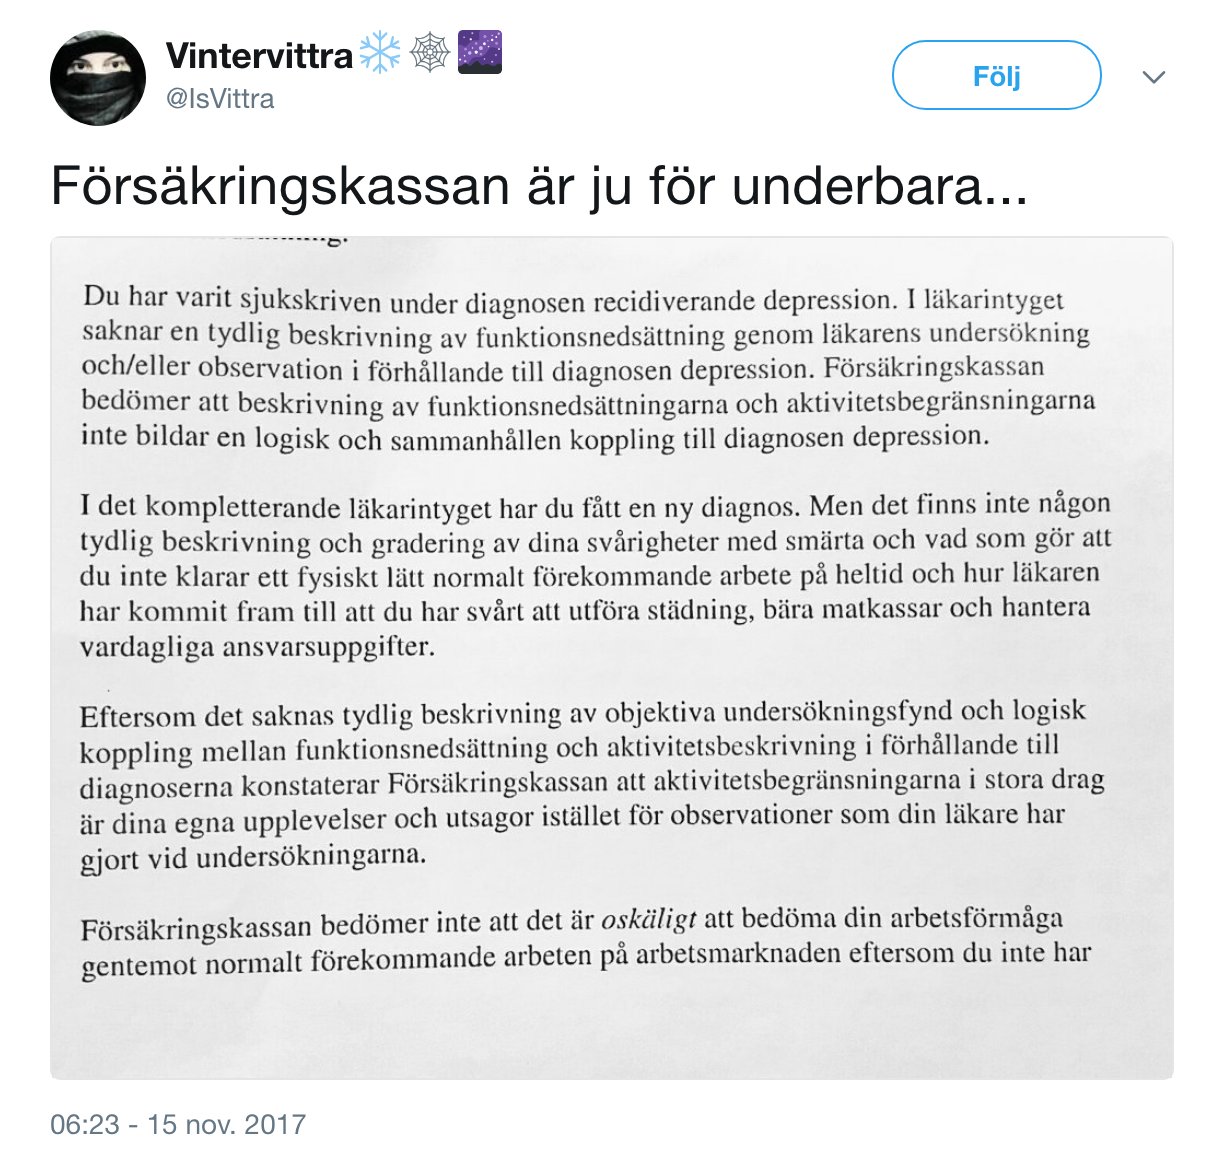
\includegraphics[width=\textwidth,height=\textheight,keepaspectratio]{930803547054239744.png}}]{15 nov 2017}{}{https://twitter.com/IsVittra/status/930803547054239744} % 930803547054239744.png är en screenshot på denna tweet då jag inte orkat transcribera..


\entry{15 nov 2017 - Maktlösheten fick läkaren Anders Jeppsson att bränna ut sig}{Ekonomer och byråkrater har tagit makten över sjukvården och låter inte dem som har kunskapen sköta jobbet, menar 65-årige läkaren Anders Jeppsson. Enligt honom har vårdpersonalen alltid haft mycket att göra. \say{I dag är det maktlösheten och inte stressen som får så många att vilja lämna sina jobb.}}{https://www.dn.se/insidan/maktlosheten-fick-lakaren-anders-jeppsson-att-branna-ut-sig/}

\entry{15 nov 2017 - Läkaren om att sjuka nekas ersättning: \say{Jag sitter på helgerna och sliter mitt hår}}{}{http://www.barometern.se/tv/arcj2h4x/}

\entry{15 nov 2017 - Fusket finns på Försäkringskassan}{I stället har man omtolkat gamla domar för att med juridiska argument kunna säga nej till människor som söker assistanshjälp. 70 procent av alla nyansökningar får nej. Människor med svåra nedsättningar förlorar sin assistans och tvingas in i komplicerade rättsprocesser. Det är en annan anledning till att de funktionshindrade tvingas anlita assistansbolag. De behöver juridisk hjälp för att klara kommunikationen med Försäkringskassan.}{https://www.aftonbladet.se/a/pa6d6}

\entry{15 nov 2017 - Regnérs reträtt om LSS inte nog}{För att klä på sig, duscha, laga mat, gå på toaletten och klara av jobbet behöver 22-åriga ölänningen Nora Eklöv hjälp. På grund av en kronisk muskelsjukdom har hon haft rätt till personlig assistans, men när hon fick arbete i Stockholm var hon tvungen att ansöka om stöd igen. Hemma på Öland hade Nora Eklöv haft rätt till 70 timmars personlig assistans i veckan. Trots det bedömde både Södermalms och Farstas stadsdelsförvaltning att Noras totala assistansbehov bara var en timme och 58 minuter i veckan.}{https://www.aftonbladet.se/a/P6Kj7}

\entry{15 nov 2017 - Debatt: Jag vill att regeringen är ärliga med vad de vill med LSS - idag säger man en sak och gör en annan}{Att som nu, hävda att funktionsnedsatta har rätt att leva som andra, ha en lagstiftning som säger att funktionsnedsatta har rätt att leva som andra men praktisera lagstiftningen som att kostnadsminskning är första prioritet är ovärdigt ett rättssamhälle och därtill moraliskt förkastligt.}{http://www.dalademokraten.se/opinion/debatt/debatt-jag-vill-att-regeringen-ar-arliga-med-vad-de-vill-med-lss-idag-sager-man-en-sak-och-gor-en-annan}

\entry{15 nov 2017}{Bara i Sverige!
Får inte tillbaka mitt körkort, har för mycket PTSD enligt Transportstyrelsen.
Försäkringskassan godkänner ej min PTSD? Trots läk. Intyg från veteranmottagningen?
Sverige är ett extremt land!
\#Veteran}{https://twitter.com/SurvivalSweden/status/930813943450423296}

\entry{15 nov 2017}{Regeringens sätt att få ner sjuktalen: dra in sjukersättningen. Den \say{svenska modellen} om man så vill. Helt bisarrt.}{https://twitter.com/GuiltyLeadfoot/status/930829955252056066}

\entry{16 nov 2017 - Enighet om att sjuka måste ha rätt till välfärden}{Allt fler och fler människor nekas sjukpenning i dagens Sverige, detta trots att läkare bedömt dem som så sjuka att de inte klarar av att arbeta.}{http://www.barometern.se/kalmar/enighet-om-att-sjuka-maste-ha-ratt-till-valfarden/}

\entry{16 nov 2017}{För det mesta hör vi bara från personer som har mått dåligt, inte folk som fortfarande är sjuka. Det ligger en sån tonvikt på att allt går över att inget annat får plats, men det går faktiskt inte alltid över. \#psykiskohälsa

\begin{quotation}
\say{I wanted to tell her that I was getting better, because that was supposed to be the narritive of illness; It was a hurdle you jumped over, or a battle you won. Illness is a story told in the past tense.}

John Green\\
\emph{Turtles All the Way Down}
\end{quotation}}{https://twitter.com/BrainBreakage/status/931405432358363137}

\entry{16 nov 2017 - Äntligen backar Regnér}{Men det är inte företag som beviljar timmarna, utan Försäkringskassan — Regnérs slag mot företagen slog i stället undan benen för de människor hon är satt att värna. Ingen drabbas som behöver hjälp, lovade Regnér. Men i snart två år har nu fyra av fem människor som för första gången söker assistans fått avslag — kostnaderna lär sluta dryga miljarden under budget. Barn med stora behov tvingas bo på sjukhus, eftersom deras läkare inte vågar släppa hem dem utan tillräcklig assistans. Kommuner planerar nya barnhem.

Maria Persdotter, ordförande Riksförbundet för Rörelsehindrade Barn och Ungdomar, säger i tidningen Leva \& Jobba med Assistans att hon ser barnhemmen som en direkt följd av att familjer inte fått assistans för sina barn.

Barnhem. Institutioner. Smaka på orden. Vuxna tvingas flytta från sina hem, föräldrar tvingas lämna sina barn ifrån sig.

Det blev allt värre. Efter en förödande dom i somras beräknades sex tusen personer förlora tidigare beviljade stödtimmar. Före nyår skulle mer än tusen människor förlora ALL den assistans som gjorde det möjligt för dem att leva, snarare än överleva. Tusen. Sex tusen.}{http://www.unt.se/asikt/debatt/antligen-backar-regnr-4820060.aspx}


\entry{16 nov 2017 - Jenny Wennberg: Regeringens besked är bara en undanmanöver}{Att regeringen inte har några andra ambitioner än att sänka antalet assistanstimmar för funktionshindrade svenskar framgår tydligt. Idag får över 80 procent av alla som söker assistans avslag på sin ansökan.

På det hela taget är det därför också en mycket ful manöver som iscensats av regeringen och som presenterades under tisdagen. Med hjälp av moratoriet försöker regeringen få bort assistansfrågan från bordet inför valet.}{http://www.dalademokraten.se/opinion/ledare/jenny-wennberg-regeringens-besked-ar-bara-en-undanmanover}


\entry{17 nov 2017}{@socialdemokrat nedskärningar inom LSS har försatt flera dövblinda föräldrar i fruktansvärd situation.

\say{Torbjörn är dövblind och pappa till två små barn. Utan hjälp får han svårt att se efter barnen. Ändå nekas han assistans.} Skandalöst. \#räddaLSS \href{https://www.facebook.com/svtteckensprak/videos/1413493768689426/?hc_ref=ARRDRaSBAF4diXGh6NZx5vBAgsvxuc_gVR1epFoVcrXwKyaUsrNNjtBfg0hJyXBw_HA}{facebook.com/svtteckensprak \ldots}}{https://twitter.com/perssontweets/status/931548119661187073}

\entry{17 nov 2017 - \say{Samhället har ett extra ansvar}}{Valdebatt. Att skära ner i rätten till personlig assistans är att dra undan mattan för tusentals familjer. Och det måste få ett slut! Det skriver Helena Hedman Skoglund (L).}{http://www.uppsalatidningen.se/insandaredebatt/samhallet-har-ett-extra-ansvar-4810094.aspx}

\entry{17 nov 2017 - Strandhäll är ingen hjälte}{Under socialförsäkringsminister Annika Strandhälls karriär har det hon sysslat med bara blivit sämre. Det är inget att hylla, skriver Zina Al-Dewany.}{http://flamman.se/a/strandhall-ar-ingen-hjalte}

\entry{17 nov 2017 - Olof förlorar nödvändig hjälp: \say{Orimligt}}{Det tog oss 16 år av kamp att få en väl fungerande hjälp. Nu slås allt i spillror, säger hans mamma Eva Ekström förtvivlat.}{http://www.barometern.se/kalmar/olof-forlorar-nodvandig-hjalp/}

\entry{18 nov 2017 - Familjens vädjan för hjärnskadade Eija}{Hon inte kan äta själv. Inte röra sig.
Hon behöver hjälp dygnet runt.
Men det räcker inte för att familjen ska beviljas särskild LSS-assistans dagtid för dottern Eija, 2,5 – född med en allvarlig hjärnskada.
Nu vänder sig pappa Mattias Isaksson, 36, direkt till barn- och hälsominister Åsa Regnér:
\say{Har du sett på när ett barn sakta dör framför dina ögon?}, skriver han på Facebook.}{https://www.expressen.se/nyheter/stockholm/hjarnskadade-eija-far-inte-lss-stod/}

\entry{18 nov 2017}{Om du tror att vi kan träna bort våra funktionsnedsättningar så har du kanske inte riktigt förstått vad en funktionsnedsättning är. \href{https://funkisfeministen.wordpress.com/2016/03/07/frustrerande-kommentarer-del-4-hen-kan-val-inte-ha-bildschema-hela-livet-heller/}{funkisfeministen.wordpress.com/2016/03/07/fru \ldots} \#skolan}{https://twitter.com/Jonna_A/status/931933216734437376}

\entry{18 nov 2017}{Jag har inte kunnat ANDAS sen avslagsbeslutet från FK sedan början av september. Varje dag och natt har jag tänkt, oroat, drömt, försökt hitta en lösning på pengar till varenda liten räkning. Jag andas nästan normalt igen när jag tänker på nästa månad.}{https://twitter.com/feministasfk/status/932022369744539649}


\entry{19 nov 2017 - Hon anklagar Försäkringskassan för psykisk misshandel: \say{Det är som om vi inte skulle vara människor}}{}{https://www.st.nu/logga-in/hon-anklagar-forsakringskassan-for-psykisk-misshandel-det-ar-som-om-vi-inte-skulle-vara-manniskor}

\entry[{
\includegraphics[width=\textwidth,height=\textheight,keepaspectratio]{DO_9zK1WAAEUcmc.jpg}}]{19 nov 2017}{Om försäkringskassan skulle ta över bilprovningen. \Emoji{😊}}{https://twitter.com/_nallen_/status/932242707044544512}

\entry{21 nov 2017 - Orolig väntan på Försäkringskassans beslut}{Omkring 1.000 personer har förlorat sin statliga personliga assistans de senaste två åren.
Familjen Klinthammar är några av dem som nu väntar oroligt på ett nytt beslut för sonen Lucas.
– Om försäkringskassan säger nej får vi sälja huset och flytta, säger pappa Johan Klinthammar.}{https://www.svt.se/nyheter/lokalt/sormland/oroligt-i-vantan-pa-forsakringskassans-beslut}

\entry{21 nov 2017 - Renée nekas sjukpenning - får sälja sina möbler}{Försäkringskassan kommer att öka avslagen på sjukpenning ytterligare. En av dem som drabbats är Renée Wåhlén.

– Det är kämpigt. Jag har sålt möbler och lånat pengar av vänner för att få ihop till mat för dagen.}{\detokenize{http://sverigesradio.se/sida/artikel.aspx?programid=93&artikel=6822864}}

\entry{21 nov 2017 - \say{Sjukförsäkringen måste ses över}}{Det här är oroväckande. Vid möten och samtal med enskilda personer och med flera fackliga organisationer, såväl TCO-förbund som LO-förbund, har det framkommit att rehabilitering av sjukskrivna har avbrutits genom indragen sjukpenning.}{https://arbetet.se/2017/11/21/sjukforsakringen-maste-ses-over/}

\entry{21 nov 2017 - Lina Norberg Juuso: Sjuka måste få vara sjuka}{Det handlar bland annat om att människor blivit nekad sjukpenning, blivit av med sin sjukpenning, tvingas att vända sig till socialförsäkringssystemet för att deras sjukdomshistoria inte passar in i mallen för att få rätt till stöd från Försäkringskassan. Det går att läsa om läkare som gör sitt yttersta för att skriva rätt sorts intyg för att deras patienter ska få sjukpenning. Det är inte klokt. Läkarnas kompetens ska användas till att ge sjuka rätt stöd, rätt behandling, rätt medicin. Inte för att få spetskompetens i snygga intyg som gillas av Försäkringskassan.}{http://www.st.nu/opinion/lina-norberg-juuso-sjuka-maste-fa-vara-sjuka}

\entry{21 nov 2017 - Välgrundad kritik mot \say{rehabiliteringskedjan}}{Det är alltså ingen tillfällighet att läkare, försäkrade, fackliga organisationer och granskande myndigheter den senaste tiden larmat om att såväl den försäkrades ekonomiska trygghet, läkarnas arbetsförhållanden som rättssäkerheten blir lidande när FK försöker uppnå det siffersatta målet.}{http://loblog.lo.se/valfard/valgrundad-kritik-mot-rehabiliteringskedjan/}

\entry{21 nov 2017 - Jag tvingas jobba – trots operation och läkarintyg}{Läkaren har skrivit tre läkarintyg och ringt till min handläggare på Försäkringskassan, ändå bedömer hon att jag kan jobba.}{http://www.vlt.se/opinion/insandare/jag-tvingas-jobba-trots-operation-och-lakarintyg}


\entry{21 nov 2017 - Utbrända Anna Hestner tar strid mot Försäkringskassan: \say{Om jag kan ge röst åt några andra så är det värt det}}{}{https://www.op.se/logga-in/utbranda-anna-hestner-tar-strid-mot-forsakringskassan-om-jag-kan-ge-rost-at-nagra-andra-sa-ar-det-vart-det}


\entry{22 nov 2017 - \say{Sjukförsäkringen inte längre rättssäker}}{Trots hård kritik har regeringen valt att behålla tidsgränserna i sjukförsäkringen. Det kombinerat med kravet på Försäkringskassan att minska antalet utbetalningar gör att sjukförsäkringen inte längre är rättssäker. Det vill vi se en ändring på, skriver LO-distriktet i Stockholms län genom ordförande Marie Jokio.}{https://arbetet.se/2017/11/22/sjukforsakringen-inte-langre-rattssaker/}

\entry[{
\includegraphics[width=\textwidth,height=\textheight,keepaspectratio]{DPUeE3UX4AAWH7G.jpg}}]{23 nov 2017}{\#intygnobbat}{https://twitter.com/AndersLinander/status/933685571372961792}

\entry{23 nov 2017 - Sjukförsäkringen - en utsorteringsmekanism}{Sjukförsäkringen har kommit att bli en utsorteringsmekansim som inte fungerar på ett rättssäkert sätt och får förödande konsekvenser för de drabbade. Enskilda personer, läkare och fackliga organisationer vittnar om stora brister i Försäkringskassans bedömningar av arbetsförmåga och rätten till ersättning. Allt fler människor får sin sjukpenning indragen till följd av Försäkringskassans hårdare bedömningar av arbetsförmågan efter regeringens uppdrag att minska sjukpenningtalet. Bedömningar som många gånger är rent oskäliga. Och som kan bidra till att den sjuke blir än sjukare.}{http://stockholm.lo.se/stockholm/uttalande_sjukforsakringen_en_utsorteringsmekanism}

\entry{23 nov 2017 - INSÄNDARE: Rop från en utbränd: Kära Försäkringskassan – ingen vill gå på knäna!}{Så kära Försäkringskassan, skippa era sunkiga och helt vidriga och omänskliga regler, se människan, ta in den individuella situationen och lyssna på vad som sägs från läkare, medmänniskor och framförallt den sjukskrivne! Ingen vill vara sjuk, ingen vill behöva gå på knäna!}{http://www.op.se/jamtland/insandare-rop-fran-en-utbrand-kara-forsakringskassan-ingen-vill-ga-pa-knana}

\entry{23 nov 2017 - Marcus kämpar för lärare som blivit sjukskrivna}{En tuff arbetssituation för lärare gör att allt fler sjukskrivs på grund av stressrelaterade åkommor – samtidigt får allt fler avslag från Försäkringskassan. Marcus Larsson, lärare i Kungälv, debatterar för de kollegor som inte orkar.}{http://kungalvsposten.se/nyheter/marcus-kampar-for-larare-som-blivit-sjukskrivna/}

\entry{24 nov 2017 - Läsartext: Vilket av partierna kan knäcka flest utsatta?}{Och jag undrar, i mitt kanske inte så jättestilla sinne, varför Socialdemokraterna kämpar så febrilt för att slå Moderaterna i kampen om vilket parti som kan knäcka flest sjuka, utsatta och skadade med sin politik?}{https://www.sydsvenskan.se/2017-11-24/vilket-av-partierna-kan-knacka-flest-utsatta}

\entry{24 nov 2017 - Svårt hjärnskadad nekas assistans: \say{Känns som en mardröm}}{Före detta Bodensarens vädjan har fått stor spridning på Facebook. Hans tvååriga dotter nekas assistans trots att hon riskerar att dö om hon inte får tillsyn dygnet runt.}{http://www.nsd.se/nyheter/svart-hjarnskadad-nekas-assistans-kanns-som-en-mardrom-nm4702240.aspx}

\entry{25 nov 2017 - Vad menar Försäkringskassan?}{Vad menas i Försäkringskassans vision? Den lyder. \say{Vår vision är ett samhälle där människor känner trygghet om livet tar en ny vändning}.

Hur tyder ni handläggare och ansvariga på försäkringskassan detta? Vad menar ni med orden trygghet och att livet tar en ny vändning? Jag undrar också över tryggheten när läkare sjukskriver mig, jag stannar hemma för att rehabiliteras och får efter två till tre veckor reda på att det övervägs att jag skall få avslag på min sjukpenning.}{http://www.ltz.se/opinion/insandare/vad-menar-forsakringskassan-1}

\entry{25 nov 2017 - Eva Lindström: Försäkringskassans attityd mot min dotter är ovärdig – och dyr}{Försäkringskassan har bestämt att hon inte längre ska jobba som sjuksköterska, utan hon uppmanas söka annat enklare jobb där hon genast kan gå in på heltid. På frågan ”Vilket annat jobb föreslår du?” får hon veta att det inte är handläggarens problem.}{https://asikt.dn.se/asikt/debatt/forsakringskassans-attityd-mot-min-dotter-ar-ovardig-och-dyr/}

\entry{25 nov 2017}{Min sjukdom klassades som arbetsskada - dfr skulle jag inte vara sjukskriven utan byta jobb. \say{Fast det gör man ju inte på en dag?!} sa jag. \say{Det är inte mitt problem} sa FK. Jag fick ta tjänstledigt istället. Och skuldsätta mig ännu mer.}{https://twitter.com/Svenska777/status/934373062027472896}

\entry{26 nov 2017 - Regeringen gör inte tillräckligt}{Det är antagligen ingen som har missat Riksförbundet för Rörelsehindrade Barn och Ungdomars (RBU) skyltar på Storgatan där det med stora bokstäver står att bara “1 av 10 får duscha”. Att bara en tiondel av de som behövde assistans blev beviljade stöd menar vi i LUF är en tragedi, och en form av diskriminering.}{http://www.smp.se/debatt/regeringen-gor-inte-tillrackligt/}

\entry{27 nov 2017 - LSS-krisen får inte begravas i en utredning}{För människor som förlorat sin personliga assistans är det slut på frihet. Situationen är allvarlig, vilket gör det orimligt att regeringen tillsätter en utredning som ska vara klar efter valet 2018. Ett snabbspår är nödvändigt, anser Liberalerna. }{https://www.dagenssamhalle.se/debatt/lss-krisen-far-inte-begravas-i-en-utredning-19648}

\entry{27 nov 2017 - Det finns ansikten bakom varenda variabel}{Det blir svårare om de som gömmer sig i slaskvariablerna får mänskliga ansikten. Om det bakom varje liten nedskärning i en formel finns en familj som går under på grund av nekad assistans eller en sönderjobbad sjuksköterska vars sargade och nyss sjukskrivna kropp måste släpa sig till jobbet igen efter att varje morgon ha svept i sig en hutt av starkt smärtstillande tabletter.}{http://www.ltz.se/opinion/ledare/det-finns-ansikten-bakom-varenda-variabel}

\entry{27 nov 2017 - Ann-Marie Begler (GD) Försäkringskassan nomineras till Årets Förvillare 2017}{Hon gick ut i radion och påstod att Försäkringskassans beslut är rättssäkra. Alla vi som i åratal försökt få dem att göra sakliga utredningar baserade på faktiska omständigheter, följa lagstiftning och beakta bevisning och läkar- och psykiatrikers utlåtanden vet att detta inte stämmer.}{http://aretsforvillare.nu/2017/11/ann-marie-begler-forsakringskassan-nomineras-till-arets-forvillare-2017/}

\entry{28 nov 2017 - LO rasar mot ökade avslag på sjukpenning}{Allt fler sjukskrivna blir av med sin sjukpenning. Sedan hösten 2015 har avslagen tredubblats och nu växer kritiken mot regeringen från de egna leden.
– De ska stå för medmänsklighet som de sa i valrörelsen. Man blir inte friskare för att man blir fattig, det här är bara en press på människor, säger Torbjörn Johansson, avtalssekreterare på LO.}{https://www.svt.se/nyheter/inrikes/lo-rasar-mot-okade-avslag-pa-sjukpenning}

\entry{28 nov 2017 - Malin förlorar sjukpenningen – trots kroniskt trötthetssyndrom}{Malin Carlbom tillbringar dagarna i en säng i ett nedsläckt rum. Fysisk belastning gör att hon får influensaliknande symtom som halsont, frossa och feber. I våras fick hon beskedet att sjukpenningen skulle dras in.
– Jag fattar inte hur det får vara så här att min läkare gör en bedömning och sedan river Försäkringskassan upp det helt och hållet, det är obegripligt, säger hon.}{https://www.svt.se/nyheter/inrikes/malin-forlorar-sjukpenningen-trots-kroniskt-trotthetssyndrom}


\entry{28 nov 2017 - Sjuka förlorar fortfarande sin sjukpenning}{I stället för att underlätta för de sjuka har regeringen snarare gasat på utförsäkringarna. Sedan socialminister Annika Strandhäll ställt kravet att sjuktalet ska pressas till i snitt nio dagar om året har Försäkringskassans avslag blivit allt fler.}{https://www.aftonbladet.se/ledare/a/4ddgkG/sjuka-forlorar-fortfarande-sin-sjukpenning}

\entry{28 nov 2017 - Om du blir sjuk – kontakta inte en läkare. Kontakta en jurist}{Men vad är det FK motsätter sig? Inte det faktum att hen är sjuk. Nej då. Dom mottsätter sig att sjukskrivningarna inte är korrekt formulerade. Har vårt socialförsäkringssystem förfallit så pass mycket att patienten måste sitta och diktera för dom ÅTTA olika läkarna som hen var tvungen att besöka under sin sjukskrivningstid för att vara berättigad till sjukpenning?}{http://tankeverket.org/politik/om-du-blir-sjuk-kontakta-inte-en-lakare-kontakta-en-jurist/}

\entry{28 nov 2017 - Fler förlorar sjukpenning – han överklagar beslut på heltid}{Regeringen får skarp kritik av LO eftersom allt fler förlorar sin sjukpenning. Mattias Åman jobbade för Metall under ett halvår enbart med att överklaga försäkringskassans beslut.}{https://www.svt.se/nyheter/lokalt/vasterbotten/jobbade-heltid-med-att-overklaga?cmpid=del:tw:20171129:jobbade-heltid-med-att-overklaga:nyh:lp}

\entry{28 nov 2017 - Strandhäll (S) vägrade debattera sjukpenningen med Sjöstedt (V)}{Allt fler sjukskrivna blir av med sin sjukpenning och kritiken mot regeringens krav på Försäkringskassan växer.
När ämnet skulle debatteras stod Annika Strandhäll (S) och Jonas Sjöstedt (V) vid varsitt bord i Aktuellts studio – något som upprört flera tittare.}{https://www.svt.se/nyheter/inrikes/strandhall-s-vagrade-debattera-sjukpenning-med-sjostedt-v}

\entry{28 nov 2017 - Alltfler sjukskriva blir av med sjukpenning}{Fler och fler sjukskrivna blir av med sin sjukpenning på grund av regeringens krav på  Försäkringskassan att pressa ner dagarna.
I kvällens Aktuellt duckar socialminister Annika Strandhäll från att debattera frågan med vänsterledaren Jonas Sjöstedt som också är inbjuden.
– Jag tycker att det här är ett sätt att smita i debatten, säger Sjöstedt.}{https://www.expressen.se/dinapengar/forsakringar/alltfler-sjukskriva-blir-av-med-sjukpenning-/}


\entry{28 nov 2017}{Har en väninna som är godeman. Det hon får lägga mest tid på nu är att strida mot FK som friskförklarar hennes klienter trots att de inte ens kan kan sköta sin egen ekonomi pga av psykoser. Hon har suttit vid mitt köksbord i en dryg timma och gråtit av vanmakt. Hur länge kommer hon orka strida för \say{sina skyddslingar}, som hon kallar dem?}{https://twitter.com/BylineBelife/status/935491716227923970}

\entry{29 nov 2017 - Vår glada dotter har brutits ner till en sorgsen människa}{Det måste kännas väldigt kränkande för alla läkare vars intyg inte gäller hos Försäkringskassan.}{http://www.st.nu/opinion/insandare/var-glada-dotter-har-brutits-ner-till-en-sorgsen-manniska}

\entry{29 nov 2017 - \say{Sjukförsäkringen en akilleshäl för S}}{Regeringens mål om sänkt sjukfrånvaro får Försäkringskassan att göra orimligt hårda bedömningar av rätten till sjukpenning. Det hävdar LO, som talar om rättsskandal.}{https://arbetet.se/2017/11/29/sjukforsakringen-en-akilleshal-for-s/}

\entry{29 nov 2017 - S-ledamöter sätter press på regeringen om sjukpenning}{Flera socialdemokrater i riksdagen motionerar för att regeringen ska göra nånting åt att allt fler nekas sjukpenning. I en motion kräver de en översyn av hur tidsgränserna i sjukförsäkringen tillämpas.}{\detokenize{http://sverigesradio.se/sida/artikel.aspx?programid=83&artikel=6832338}}

\entry{29 nov 2017 - Vad hände med löftena om sjukförsäkringen?}{Inför valet 2014 stod frågan om sjukförsäkringen högt uppe på den politiska dagordningen. Många personer vittnade om svårigheterna att få ersättning, om underkännanden av sjukintyg från läkare, hur de föll mellan stolar då de var för sjuka för att jobba men för friska för att vara sjuka. Många berättade om utförsäkring och om skammen över att inte kunna försörja sig. Frågan engagerade många och löftena om en bättre och mer täckande sjukförsäkring kom från flera håll.}{http://www.lo.se/start/seminarium/vad_hande_med_loftena_om_sjukforsakringen}

\entry{29 nov 2017 - Ledare: Pendeln har svängt för långt. Justera sjukvillkoren.}{Och visst hamnar människor i kläm – men inte i första hand mellan olika myndigheter, utan snarare mellan verkligheten och de politiska målen.}{https://www.sydsvenskan.se/2017-11-29/pendeln-har-svangt-for-langt-justera-sjukvillkoren}

\entry{30 nov 2017 - \say{Vad är regeringens definition av human sjukförsäkring?}}{Istället för att målet är just det, - ett mål, blir det ett tak. Och för att inte spräcka de övre nivåerna (som nio dagar i sjukpenningtaket eller 18.000 personer med sjukersättning och år) väljer man att helt enkelt inte bevilja sjukskrivna ersättning.}{https://www.folkbladet.nu/1971212}

\entry{30 nov 2017 - Sluta jaga de sjukskrivna}{Regeringen har målet att pressa ner sjuktalen. Det är i grunden en positiv målsättning, men den får inte gå över till en hetsjakt på sjuka. Dessvärre kommer allt fler exempel på att Försäkringskassan går för hårt fram.}{https://www.vf.se/ledare/sluta-jaga-de-sjukskrivna/}

\entry{1 dec 2017}{2,5 år utan en krona. AF slängde ut mig med för jag är för sjuk. Tycker du att FK tagit ett noggrant beslut? @strandhall \#mellanstolarna \#FK}{https://twitter.com/KidsAreFuture/status/936573538873602048}

\entry{1 dec 2017}{Snälla @strandhall jag orkar inte mer. Jag orkar inte ännu en förtvivlad kommunalarbetande äldre kvinna, med söndervärkt kropp som fått avslag från Försäkringskassan som gråter i telefon. Jag slits itu över att jag som @FacketKommunal inte kan hjälpa henne mot orättvisan.}{https://twitter.com/LoanSundman/status/936652052901580800}

\entry{2 dec 2017 - Zandra, 29, har MS – kan inte leva av aktivitetsstödet: \say{Det är en enorm stress}}{Det finns inte en person som kan svara på alla frågor, utan jag hänvisas hela tiden runt till olika personer och enheter på Försäkringskassan, berättar hon. Nu har Zandra lämnat in ansökan om socialbidrag. – Det är det som återstår. Vad har vi för trygghetssystem i det här landet när en ung människa \ldots}{https://www.allehanda.se/logga-in/zandra-29-har-ms-kan-inte-leva-av-aktivitetsstodet-det-ar-en-enorm-stress}

\entry{2 dec 2017 - Peter Boström: Bättre koll på bilar än människor}{Det kallas Försäkringskassan. Försäkringskassan gör allt det som bilprovningen gör med bilar, fast med människor - och tvärtom. Den som 2017 rullas in vid Försäkringskassan behöver inte direkt vara orolig för att blir utdömd. På Försäkringskassan 2017 stämplas alla som antingen fullt eller i vart fall delvisa körbara. En människokropp tycks vara mindre noggrann att reparera, hålla under uppsikt och låta vila, i alla fall än en normalsliten bil med taskiga mönsterdjup och dåliga bromsskivor.}{http://www.olandsbladet.se/asikter/peter-bostrom-battre-koll-pa-bilar-an-manniskor/}

\entry{2 dec 2017 - De svagaste får ta mest
 stryk}{\say{Någonstans runt 15 000 personer i landet berörs av Försäkringskassans tolkningar av de domar som tagits i Högsta förvaltningsdomstolen. Det som drabbar dem är ett oerhört stort lidande. Det är ett hån. Det är ett straff.}

Att andas är inget grundläggande behov. Eller att över huvud taget kunna klara sin vardag. Det har tusentals personer i landet fått veta, när deras personliga assistans har blivit indragen.}{http://www.barometern.se/debatt/de-svagaste-far-ta-mest-stryk/}

\entry{2 dec 2017 - Den inhumana sjukförsäkringen – Varför ministern inte vågar ta debatten}{Varför vill inte Annika Strandhäll debattera sjukförsäkringen med Jonas Sjöstedt? Svaret är så enkelt som att hon vet att vår beskrivning är sann men att hon också vet att hon inte kan inte säga det. Det skulle syna regeringens bluff om att de hanterat problemet med allt sämre arbetsmiljö i vård, skola och omsorg och det skulle bli tydligt att de vallöften som gavs i valrörelsen 2014 inte uppfyllts, utan att Socialdemokraterna i praktiken gjort det lättare att utförsäkra sjuka.}{http://tankesmedjanbalans.se/den-inhumana-sjukforsakringen-varfor-ministern-inte-vagar-ta-debatten/}

\entry{3 dec 2017 - S måste sluta slå sönder funktionshindrades liv}{Trots att samhällets gemensamma resurser växer så väljer den nuvarande rödgröna regeringen att acceptera miljardbesparingar på det statliga stödet till personer med funktionsnedsättningar.}{http://www.gp.se/nyheter/debatt/s-m%C3%A5ste-sluta-sl%C3%A5-s%C3%B6nder-funktionshindrades-liv-1.4884989}

\entry{3 dec 2017 - LSS-manifestation lockar partiledare}{Alla ska ha rätt till personlig assistans. Det är budskapet under helgens manifestation på Norra Bantorget. Ebba Busch Thor (KD), Jan Björklund (L), Jonas Sjöstedt (V) och ett tusental andra väntas delta.}{https://www.dn.se/sthlm/lss-manifestation-lockar-partiledare/}

\entry{3 dec 2017 - Birgitta: Tack vare assistans lever min son ett bra liv}{Runt om i landet sker manifestationer för att slå ett slag för den personliga assistansen. För andra året i rad så äger manifestationen \say{Rädda LSS, assistans är frihet} rum.}{\detokenize{http://sverigesradio.se/sida/artikel.aspx?programid=87&artikel=6833323}}

\entry{3 dec 2017 - Demonstrationer för att behålla rätten till assistans}{I dag, söndag, anordnas manifestationer över hela landet för att demonstrera mot att personer i Sverige har förlorat rätten till personlig assistans.
– Jag är beroende av assistans för att leva som en fullvärdig medborgare, säger Gillan Andersson, en av demonstranterna.}{https://www.svt.se/nyheter/demonstrationer-for-att-behalla-ratten-till-hjalp}

\entry{3 dec 2017 - En mors fruktlösa kamp}{Ofta, ofta, ringer Berit upp mig. Hon orkar inte mer säger hon, gråtandes. Berits fruktlösa kamp för sin vuxna dotters vård inom psyk börjar nå sitt slut. Berit har kämpat sig slut, fysiskt sjuk, med en möjlig halstumör nyligen upptäckt. Hon säger att den kom för att hennes röst är tystad.}{https://www.patientperspektiv.org/en-mors-fruktlosa-kamp/}

\entry{3 dec 2017}{Jag kan,oförmögen som jag är,bara nå en slutledning. Det är inte okej att vara sjuk i Stefan löfvens ( @SwedishPM ) Sverige. Det är budskapet som basuneras ut från Rosenbad.}{https://twitter.com/BUT7MAN/status/937306285099413506}

\entry{3 dec 2017 - Var finns visionerna i dagens socialpolitik?}{I valrörelsen 2018 kan man inte göra valaffischer på målet om nio dagars sjukersättning per löntagare. Det är ingen paroll som kommer att leda till entusiasm ute bland människorna. Inte heller att en multisjuk sedan 2008 ska söka heltidsjobb.}{http://www.ltz.se/opinion/ledare/var-finns-visionerna-i-dagens-socialpolitik}


\entry{3 dec 2017 - Kostnaderna för sjukförsäkringen har skenat enormt – dags för en haveriutredning}{Som läkare har jag med stigande vanmakt och frustration fått se både patienter och vänner fara oerhört illa av Försäkringskassans handläggnings- och beslutssystem. De effekter ett beslut om avslag på ersättning har för svårt sjuka och funktionshindrade människors psykiska mående främjar varken tillfrisknandet eller påskyndar återgången till arbete. Tvärtom.

Funktionsnivån sänks ytterligare av depression, ångest, känslor av uppgivenhet, vanmakt och hopplöshet. Och i värsta fall kanske ger man upp helt. Och handen på hjärtat – hur många psykiskt sjuka patienter klarar att inkomma med synpunkter eller överklaga Försäkringskassans beslut. De få som klarar av det, finner allt som oftast att deras yttrande lämnas utan kommentar.}{http://www.st.nu/opinion/insandare/kostnaderna-for-sjukforsakringen-har-skenat-enormt-dags-for-en-haveriutredning}

\entry{4 dec 2017 - Allvarligt sjuka nekas sjukpenning}{Jan Johansson krockade i tjänsten och blev några år senare påkörd av en drogpåverkad bilist. Trots flera svåra skador har han förlorat sin sjukpenning och ska klara ett \say{normalt förekommande arbete}, enligt Försäkringskassan. Nu ska myndighetens hårda bedömning av sjukskrivnas arbetsförmåga prövas av Högsta förvaltningsdomstolen.}{https://www.arbetarskydd.se/tidningen/allvarligt-sjuka-nekas-sjukpenning-6886365}

\entry{4 dec 2017 - Fackets ilska mot sossarna behövs}{Regeringens krav att pressa ner sjukskrivningarna är det som gör att avslagen ökar. Torbjörn Johansson beskriver för SVT hur Försäkringskassans hantering håller på att haverera när svårt sjuka plötsligt definieras som friska.

Försäkringskassan själv menar att det är bättre kvalitet i utredningarna som gör att de lyckas pressa ner siffrorna.

Men berättelserna från verkligheten beskriver motsatsen.}{http://nsd.se/nyheter/fackets-ilska-mot-sossarna-behovs-nm4707447.aspx}

\entry{4 dec 2017}{\say{Här har man arbetat och betalt in skatt i 30 år till sjukförsäkringen men nu när jag är utbränd får jag inte möjlighet att bli bra.}

En klient som i telefon berättar om FK:s rigida sjukskrivningsvägran som leder till att stressade människor blir ännu mer stressade.}{https://twitter.com/HenrikLundSALO/status/937620074382479360}

\entry{4 dec 2017}{Snart sagt varenda S-märkt ledarsida har insett den bisarra verkligheten, men regeringen låtsas som att det regnar.}{https://twitter.com/TornbergHakan/status/937644799074631680}

\entry{4 dec 2017}{Jag undrar varför jag måste ägna tid åt att förklara för Försäkringskassan varför mina cancerpatienter under pågående cellgiftsbehandling behöver sjukskrivning, men det är enl @strandhall ok att \say{sjukskriva sig} när man inte klarar av det som rimligen ingår i ett chefsjobb?}{https://twitter.com/anmariaiglesias/status/937922567670726656}

\entry{4 dec 2017 - Erland tog sitt liv dagen efter beskedet att han inte fick vara sjukskriven}{Erland levde med konstant smärta. Precis när det började finnas hopp om ett mer smärtfritt liv nekade försäkringskassan hans fortsatta sjukskrivning. Dagen efter beskedet beger Erland sig ut i skogen och begår självmord.}{https://www.op.se/jamtland/erland-tog-sitt-liv-dagen-efter-beskedet-att-han-inte-fick-vara-sjukskriven}

\entry{5 dec 2017 - Pappers: S ska inte jaga sjuka och sköra}{Det är med stor besvikelse vi ser hur de hårda tagen mot sjuka och sköra människor fortsätter och till och med förvärras under den rödgröna regeringen. Stoppa jakten på de sjuka och börja bekämpa ohälsan istället, skriver Matts Jutterström, ordförande i Pappers.}{http://www.dagensarena.se/opinion/pappers-s-ska-inte-jaga-sjuka-och-skora/}

\entry{5 dec 2017 - Det välmående Sverige stämmer inte}{Det är inte roligt att prata med gråtande familjer som fått hela sina liv upp- och nedvända efter de nya LSS-reglerna.}{http://www.olandsbladet.se/asikter/det-valmaende-sverige-stammer-inte/}

\entry{5 dec 2017 - Att stå utan pengar till mat och hyra gör ingen människa frisk}{Regeringen vill minska sjukdagarna generellt i Sverige säger de. Då människor inte slutar bli sjuka och utslitna inom vård, skola och omsorg så finns det bara ett sätt för Försäkringskassan att nå det av regeringen utsatt målet som är 9.0 dagar per år och vuxen arbetare. Detta kan bara nås genom att ge avslag på sjukpenningsansökan.}{http://www.politism.se/story/att-sta-utan-pengar-till-mat-och-hyra-gor-ingen-manniska-frisk/}

\entry{5 dec 2017 - Läkare kritisk till Försäkringskassans hårdare regler}{Han beskriver situationen som en översvämning och gör liknelsen med en fördämningsdamm.

— Det känns som de stänger dammluckorna för att dämma upp sjukskrivningsfloden. Sen blir de överraskade av att det svämmar över och ledsna över att folk drunknar.}{https://www.op.se/jamtland/ostersund/lakare-kritisk-till-forsakringskassans-hardare-regler}

\forloop[-1]{entrycnt}{\theentrycnt}{\theentrycnt > 0}{
	\makeentry{\theentrycnt}
}

\end{document}
